% =========================================================================
%  Constructive Gauges — preprint
%  Compile with: xelatex (required for fontspec / unicode-math)
%  Standard: K.R. Ryan trilogy preprint template (matches Parasitic Liquidity)
% =========================================================================

\documentclass[11pt,a4paper]{article}

% Fonts: TeX Gyre Termes (Times equivalent) with matching math
\usepackage{fontspec}
\usepackage{unicode-math}
\setmainfont{texgyretermes}[
  Extension      = .otf,
  UprightFont    = *-regular,
  BoldFont       = *-bold,
  ItalicFont     = *-italic,
  BoldItalicFont = *-bolditalic,
]
\setmathfont{texgyretermes-math.otf}
\frenchspacing

% Body size / leading: 11.5pt / 13.5pt
\makeatletter
\renewcommand{\@xpt}{11.5}
\renewcommand{\@xiipt}{13.5}
\renewcommand\normalsize{%
  \@setfontsize\normalsize\@xpt\@xiipt
  \abovedisplayskip 10\p@ \@plus2\p@ \@minus5\p@
  \abovedisplayshortskip \z@ \@plus3\p@
  \belowdisplayshortskip 6\p@ \@plus3\p@ \@minus3\p@
  \belowdisplayskip \abovedisplayskip
  \let\@listi\@listI}
\makeatother
\normalsize

% Page layout
\usepackage[margin=1in]{geometry}
\setlength{\headheight}{14pt}

% Math
\usepackage{amsmath,amsthm}

% Tables
\usepackage{array}
\usepackage{booktabs}
\usepackage{longtable}
\usepackage{ragged2e}
\newcolumntype{L}[1]{>{\RaggedRight\arraybackslash}p{#1}}
\setlength{\extrarowheight}{2pt}

% Float placement
\usepackage{float}

% Captions: Fig./Table. with period separator, label at footnotesize
\usepackage{caption}
\captionsetup{figurename=Fig.,labelsep=period,margin=1.2cm,labelfont=footnotesize}

% Lists (tight, indented)
\usepackage{enumitem}
\setlist{leftmargin=1.2cm,labelindent*=.6cm,itemsep=0cm,parsep=0cm,topsep=0cm}

% Prevent orphaned headings
\usepackage{needspace}

% Section heading style (lighter than article default)
\usepackage{titlesec}
\titleformat{\section}[block]{\fontsize{13pt}{15pt}\bfseries}{\thesection.}{0.6em}{}
\titlespacing*{\section}{0pt}{18pt}{8pt}
\titleformat{\subsection}[block]{\fontsize{11.5pt}{13.5pt}\bfseries\itshape}{\thesubsection.}{0.6em}{}
\titlespacing*{\subsection}{0pt}{14pt}{6pt}

% Graphics + TikZ + pgfplots
\usepackage{graphicx}
\usepackage{tikz}
\usetikzlibrary{positioning,arrows,calc,patterns}
\usepackage{pgfplots}
\pgfplotsset{compat=1.18}

% Paragraph rules: indented first line, no gap, indentfirst on
\usepackage{indentfirst}
\emergencystretch=1em
\widowpenalty=10000
\clubpenalty=10000

% Float / display-math spacing
\setlength{\intextsep}{8pt plus 2pt minus 2pt}
\setlength{\floatsep}{8pt plus 2pt minus 2pt}
\setlength{\textfloatsep}{10pt plus 2pt minus 2pt}
\AtBeginDocument{%
  \setlength{\abovedisplayskip}{18pt plus 3pt minus 2pt}%
  \setlength{\belowdisplayskip}{18pt plus 3pt minus 2pt}%
  \setlength{\abovedisplayshortskip}{14pt plus 2pt minus 1pt}%
  \setlength{\belowdisplayshortskip}{14pt plus 2pt minus 1pt}%
}

% Tables: 1.2 row stretch, content at \small
\renewcommand{\arraystretch}{1.2}
\AtBeginEnvironment{tabular}{\small}

% Microtype refinement
\usepackage{microtype}

% Citations: superscript numeric, baseline labels in bibliography
\usepackage[superscript,biblabel]{cite}

% Bibliography: hanging indent with the label sitting in its own column
% (entries at 10pt with 6pt vertical gap)
\makeatletter
\renewenvironment{thebibliography}[1]
  {\section*{\refname}%
   \fontsize{10pt}{12pt}\selectfont
   \list{\@biblabel{\@arabic\c@enumiv}}%
        {\settowidth\labelwidth{\@biblabel{#1}}%
         \leftmargin\labelwidth
         \advance\leftmargin-0.8em
         \advance\leftmargin\labelsep
         \setlength\itemindent{1em}%
         \setlength\itemsep{6pt plus 1pt minus 1pt}%
         \setlength\parsep{0pt}%
         \usecounter{enumiv}%
         \let\p@enumiv\@empty
         \renewcommand\theenumiv{\@arabic\c@enumiv}}%
   \sloppy\clubpenalty4000\widowpenalty4000\sfcode`\.\@m}
  {\def\@noitemerr{\@latex@warning{Empty `thebibliography' environment}}%
   \endlist}
\makeatother

\usepackage{etoolbox}

% Abstract: 10pt/13pt, run-in "Abstract." lead, inset 0.5in each side
\renewenvironment{abstract}{%
  \fontsize{10pt}{13pt}\selectfont
  \begin{list}{}{%
    \setlength{\leftmargin}{0.5in}%
    \setlength{\rightmargin}{0.5in}%
    \setlength{\listparindent}{0pt}%
    \setlength{\parsep}{6pt plus 2pt minus 1pt}%
    \setlength{\topsep}{0pt}%
    \setlength{\partopsep}{0pt}%
  }\item[]\noindent\textbf{Abstract.}\hspace{0.5em}\ignorespaces
}{\end{list}}

% Colours
\usepackage{xcolor}

% Hyperlinks + PDF metadata
\usepackage{hyperref}
% Forbid mid-URL line breaks (split URLs extract as broken references on SSRN;
% see programme tracker C26). Applied 2026-07-22.
\def\UrlBreakPenalty{10000}
\def\UrlBigBreakPenalty{10000}
\hypersetup{
  colorlinks=true,
  allcolors=blue!50!black,
  pdfauthor={K.R. Ryan},
  pdftitle={Constructive Gauges: Remediating Parasitic Liquidity in Concentrated Liquidity Emissions},
  pdfsubject={Concentrated liquidity gauge design and emission distribution},
  pdfkeywords={automated market maker, ve(3,3), reward accumulator design, mechanism design}
}

% Running header (author left, page number centred footer)
\usepackage{fancyhdr}
\pagestyle{fancy}
\fancyhf{}
\fancyhead[L]{\small\itshape K.R.\ Ryan}
\fancyhead[R]{}
\fancyfoot[C]{\thepage}
\renewcommand{\headrulewidth}{0pt}
\fancypagestyle{plain}{%
  \fancyhf{}%
  \fancyfoot[C]{\thepage}%
  \renewcommand{\headrulewidth}{0pt}%
}

% Theorem environments (default amsthm styles)
\renewcommand\qedsymbol{\ensuremath{\mdlgblksquare}}
\theoremstyle{definition}
\newtheorem{definition}{Definition}
\theoremstyle{plain}
\newtheorem{theorem}{Theorem}
\newtheorem{lemma}{Lemma}
\newtheorem{corollary}{Corollary}
\newtheorem{proposition}{Proposition}
\theoremstyle{remark}
\newtheorem{remark}{Remark}

% Code-block environment (cream-tinted, footnotesize)
\usepackage{mdframed}
\newenvironment{codeblock}{%
  \begin{mdframed}[%
    backgroundcolor=brown!3!white,%
    linewidth=0pt,%
    innertopmargin=6pt,%
    innerbottommargin=6pt,%
    innerleftmargin=12pt,%
    innerrightmargin=12pt,%
    leftmargin=0.075\linewidth,%
    rightmargin=0.075\linewidth,%
    skipabove=6pt,%
    skipbelow=6pt%
  ]\footnotesize%
}{%
  \end{mdframed}%
}

% Paragraph spacing: indented first line, no gap between paragraphs
\setlength{\parindent}{18pt}
\setlength{\parskip}{0pt}

% =========================================================================
\begin{document}
\sloppy
\thispagestyle{plain}

% --- TITLE BLOCK ----------------------------------------------------------
\begin{center}
{\fontsize{10pt}{12pt}\selectfont WORKING PAPER}\\[6pt]
{\huge Constructive Gauges:\\[6pt]
Remediating Parasitic Liquidity\\[4pt]
in Concentrated Liquidity Emissions}

\vspace{14pt}
{\large K.R.\ Ryan}\\[4pt]
{\fontsize{9pt}{11pt}\selectfont Independent Researcher \quad|\quad ORCID - 0009-0004-6295-7040 \quad|\quad \href{mailto:gancor@gancor.xyz}{gancor@gancor.xyz}}\\[4pt]
{\fontsize{9pt}{11pt}\selectfont April 2026}

\vspace{12pt}
{\fontsize{9pt}{11pt}\selectfont
\begin{minipage}{0.82\linewidth}\centering
\textbf{Keywords}\hspace{0.6em}automated market maker \textperiodcentered\ ve(3,3) \textperiodcentered\ reward accumulator design \textperiodcentered\ mechanism design\\[4pt]
\textbf{JEL:} G14, G19, G23, D47
\end{minipage}}
\end{center}

% --- Therefore-symbol divider ---------------------------------------------
\vspace{-1pt}
\centerline{\scalebox{1.5}{$\therefore$}}
\vspace{14pt}

% --- ABSTRACT (single paragraph; run-in "Abstract." lead automatic) -------
\begin{abstract}
This paper identifies and corrects a measurement gap in ve(3,3) concentrated liquidity gauges. The Synthetix reward accumulator distributes voter-directed emissions in proportion to instantaneous staked liquidity, while the protocol intends to incentivise sustained tradeable depth. That gap admits the parasitic extraction vector of\cite{ryan2026c}, in which a position satisfying gauge staking conditions can collect emissions without serving a swap. \emph{Constructive gauges} close the gap by attaching three multiplicative factors to each position's nominal liquidity, a concentration weight non-increasing in range width, a freshness weight non-increasing in time-since-rebalance, and an in-range indicator. Three theorems characterise the framework. Theorem~1 bounds the ratio of corrective to standard-gauge parasitic revenue by a freshness ratio times a concentration ratio, under a Brownian log-price in the large-population mean-field regime. Theorem~2 gives the analogous equality for legitimate-LP yield. Theorem~3 shows that any proper subset of the three factors reopens at least one of the short-cycle, out-of-range, and width-arbitrage pathways, without invoking the price model or population statistics. A Foundry fork-test suite exercises the accumulator against live Aerodrome Slipstream state on Base, with cross-chain replications on PancakeSwap V3, Thena FUSION, and Ramses V2. The Gaussian in-range probability is checked against 24-hour tick traces from two Aerodrome CL100 pools; empirical departures at multi-hour horizons leave the parasitic bound conservative. Calibration against 94{,}469 rebalance events across 48 pools (a single-operator dataset, 7~March to 13~April 2026) sets a warmup window of 10 to 30 seconds.
\end{abstract}

% ---- 1. Introduction ----
\section{Introduction}\label{sec:intro}

Concentrated liquidity gauges in ve(3,3) protocols pay emissions in proportion to staked liquidity at the active tick, instant by instant, on the Synthetix \texttt{rewardPerToken} accumulator\cite{synthetix2019,egorov2019}. The accumulator was designed for fungible-token staking, where stake share equals tradeable-depth share. Under concentrated liquidity\cite{adams2021} the two diverge: a position can sit at the active tick without serving swaps, and can sit there only briefly. The accumulator therefore pays for nominal stake rather than the depth that voters directed emissions towards.

The divergence matters because ve(3,3) emissions are a voter-directed subsidy\cite{cronje2022}. The inflation budget is allocated across pools by veNFT votes, with the subsidy intended to attract real liquidity to voted pools. When the accumulator pays for nominal stake rather than tradeable depth, positions satisfying gauge staking conditions without serving swaps collect the subsidy regardless. The resulting parasitic-liquidity vector\cite{ryan2026c} admits, at the limit, a minimum-width position deposited and withdrawn across a single block, earning emissions without ever being present for a swap.

In April 2026, decoded \texttt{Mint}/\texttt{Burn}/\texttt{Stake}/\texttt{Swap} sequences across 15 Aerodrome Slipstream pools showed the strategy operating at production scale (decoder script and block range in Appendix~\ref{app:reproduction}). Of the operator-staked blocks observed in that sample, $93.6\%$ contained zero \texttt{Swap} events on the same pool, and every position except one used minimum tick spacing; Flashblocks sub-block ordering compressed the operator's wall-clock impermanent loss exposure per cycle while leaving the per-block reward basis unchanged, since the accumulator advances on \texttt{block.timestamp} between parent blocks. The pattern is not Flashblocks-specific. BSC and Arbitrum gauges built on the same accumulator template are exposed to the same strategy.

Prior remediations, a minimum position width and a reward warmup period\cite{ryan2026c}, each address one of three enabling properties (duration, width, utilisation). They are effective in combination but do not specify how emission rewards should be distributed across heterogeneous positions in a concentrated liquidity pool. I propose a scoring function for that distribution. Within the product-form family over the three corrections, the full three-factor scoring is the only member that closes the three pathways of Definition~\ref{def:pathways} (Theorem~\ref{thm:mincomplete}). The \emph{parasitic extraction ratio bound} (Theorem~\ref{thm:parasitic}) bounds the ratio of corrective to standard-gauge parasitic revenue under a steady-state legitimate population. The \emph{legitimate-LP yield equality} (Theorem~\ref{thm:legit}) gives the matching equality for legitimate LPs at arbitrary cadence. The minimal-completeness result is the only one that does not invoke the price model or population statistics.

The paper sits within a research programme on concentrated liquidity mechanism design. \emph{The Geometric Siphon}\cite{ryan2026a,ryan2026b} formalises the capital flow primitive that emerges from atomic rebalancing of concentrated liquidity positions. \emph{Parasitic Liquidity}\cite{ryan2026c} identifies the emission extraction vector this paper closes, verifies it on Slipstream CL gauges and PancakeSwap MasterChefV3 on Base, and proposes the minimum-width and warmup remediations the present scoring function generalises.

A Foundry fork-test suite exercises the corrective accumulator against live Aerodrome Slipstream state on Base, with cross-chain replications on PancakeSwap V3, Thena FUSION, and Ramses V2 reproducing the qualitative properties on three independent codebases. Lemma~\ref{lem:pin}'s Gaussian in-range probability is validated against tick traces from two Aerodrome pools; empirical $\bar P_{\text{in}}$ exceeds the Gaussian at multi-hour horizons, leaving the parasitic bound on the safe side. Parameters are calibrated against a single-operator dataset of 94{,}469 rebalance events across 48 pools over a 38-day pre-migration window; under the calibrated reference instance, the extraction bound from Cor~\ref{cor:short} evaluates to a small multiple of $c(w_{\min})/c_{\text{ref}}$ at the 2-second cycle scale (\S\ref{sec:calibration}).

Section~\ref{sec:related} places the paper in the V3 LP economics literature. Section~\ref{sec:background} introduces the standard accumulator and the three enabling properties. Section~\ref{sec:framework} states the corrective scoring function. Section~\ref{sec:analysis} gives the formal results, with full derivations collected in Appendix~\ref{app:derivations}. Section~\ref{sec:empirical} summarises the Foundry suite and the in-range probability validation, with test descriptions in Appendix~\ref{app:forkmap}. Section~\ref{sec:calibration} reports the operational calibration. Section~\ref{sec:discussion} discusses incentive compatibility, the architectural framing within ve(3,3), and limitations. Section~\ref{sec:conclusion} concludes.

% ---- 2. Related work ----
\section{Related work}\label{sec:related}

Three lines of work intersect this paper: V3 LP economics, ve(3,3) emission allocation, and CL-gauge security. Heimbach \emph{et al.}\cite{heimbach2022} document wide dispersion in V3 LP widths and lifetimes, with only actively managed positions earning non-trivial returns; the dataset in \S\ref{sec:calibration} sits in that tail. Hasbrouck \emph{et al.}\cite{hasbrouck2025} model V3 CL provision as a covered call sold at intrinsic rather than market value, supplying the canonical economic framework for the LP-population analysis underlying \S\ref{sec:legit-thm}. Cartea \emph{et al.}\cite{cartea2024} formalise \emph{concentration risk} as a determinant of optimal range width; the $c(w)$ factor of~(\ref{eq:score}) is the gauge-side analogue, rewarding the sustained concentration that legitimate LPs already optimise for. The loss-versus-rebalancing framework of Milionis \emph{et al.}\cite{milionis2022b} supplies the Brownian log-price model used in \S\ref{sec:analysis}. On ve(3,3) emission allocation, Lloyd \emph{et al.}\cite{lloyd2023} document empirically that bribe markets are a primary determinant of veToken allocation across pools; what happens within a pool, after voters have directed emissions to it, is the layer this paper addresses. The parasitic vector is distinct from the just-in-time attack of Xiong \emph{et al.}\cite{xiong2023}, which captures fees around a single swap rather than emissions over the accumulator.

Spearbit's November 2023 security review of Slipstream's concentrated liquidity implementation\cite{spearbit2023} noted that the reward accumulator may be gameable on chains with a mempool, described a claim-unstake-JIT-restake loop, and recommended evaluating whether a volume-based reward system would be fairer than the time-based accumulator; the issue was acknowledged, with monitoring rather than redesign proposed. The present work formalises a more general strategy space that does not require mempool visibility (\S\ref{sec:empirical}) and specifies a corrective scoring function tracking tradeable depth, calibrated against actively managed legitimate-LP cadence in the dataset of \S\ref{sec:calibration}.

Within the ve(3,3) CL gauges I have inspected at the contract level for this paper (Velodrome, Aerodrome Slipstream, Ramses V2, Pharaoh, Shadow, Thena V3.3, with specific revisions and source pointers in Appendix~\ref{app:reproduction}), the per-LP reward math reduces to the Synthetix \texttt{rewardPerToken} / \texttt{earned} pattern on tick presence: Velodrome, Aerodrome, Ramses, Pharaoh, and Shadow operate on per-position liquidity via \texttt{rewardGrowthInside}, and Thena V3.3 operates on fungible ERC20 wrappers of managed CL positions via the same Synthetix template. None of the inspected revisions weight by position width, time since deposit, or realised volume at that layer. I do not claim coverage of revisions outside that set. Thena's V3.3 upgrade (May 2025) was announced with performance-framing marketing, but its active emission distribution runs through Synthetix gauges rather than the Algebra farming layer, whose \texttt{factory.farmingAddress()} pointer shows zero event logs across sampled windows from mid-2025 onwards.

Two deployed systems implement partial analogues. Algebra's eternal farming exposes an optional \texttt{minimalPositionWidth} parameter, used by QuickSwap on Polygon incentives at five times tickSpacing, a direct analogue of the step-function minimum-width remediation of\cite{ryan2026c}. QuickSwap is not a ve(3,3) protocol, so the decoupling problem this paper targets does not arise in the same form there, but its use demonstrates that minimum-width admission works in production on Algebra-powered CL. Slipstream-family gauges have no equivalent built-in. Merkl by Angle Labs\cite{merkl2023} distributes rewards off-chain via a time-weighted liquidity-contribution factor rewarding ``sustained concentration over time, not short-term volume or swap activity'', a conceptual analogue of the combined concentration and freshness factors here, but operates at the reward-distribution layer with off-chain computation and optimistic verification rather than on-chain at the gauge scoring function. Merkl's weights are also independently configurable per campaign without a minimality argument that all factors must be non-zero; Theorem~\ref{thm:mincomplete} provides that minimality.

No deployed gauge inspected for this paper composes graded concentration, freshness, and an in-range factor at the LP-measurement layer, and none offers a minimality argument analogous to Theorem~\ref{thm:mincomplete}.

% ---- 2. Background ----
\section{Background}\label{sec:background}

\subsection*{Operational terms}

A position's \emph{tradeable depth} on a cycle is the in-range concentrated liquidity it contributes at the active tick over that cycle, weighted by how long it is held within the cycle; this is the quantity that absorbs incoming swaps and the quantity ve(3,3) emissions are intended to subsidise. A position is \emph{legitimate} when $w \geq w_{\min}$, $\rho \geq W$, and the position is held statically over its rebalance interval $[0, \rho]$. The set of legitimate positions in a pool is the \emph{legitimate-LP population}, against which $c_{\text{ref}}$ and $f_{\text{eq}}$ are measured and against which Theorem~\ref{thm:legit} reports yield.

\subsection{The three enabling properties}\label{sec:properties}

The standard gauge reward formula is
\begin{equation}
\text{reward}_i \;=\; \text{rewardRate} \cdot \underbrace{\Delta t}_{\text{duration}} \cdot \underbrace{\frac{L_i}{\sum_j L_j}}_{\substack{\text{width} \\ \text{utilisation}}}
\end{equation}
with $L_i$ position $i$'s liquidity at the active tick. Three properties drive the vulnerability\cite{ryan2026c}. The \emph{duration} property is that $L_i$ is a point-in-time value with no time-averaging or minimum-duration component. The \emph{width} property is that a minimum-width position earns the same rate per unit of liquidity as a position of any wider range. The \emph{utilisation} property is that emissions accrue for mere presence at the active tick; concentrated liquidity gauges already filter out-of-range positions through the range-aware per-position accumulator, but an in-range position earns irrespective of actual swap volume served.

The duration property enables short-cycle extraction, the utilisation property enables out-of-range accrual on gauges without range-aware accumulators, and the width property enables width arbitrage (Definition~\ref{def:pathways}). Closing a property closes the corresponding pathway.

\subsection{Limitations of existing remediations}\label{sec:insufficient}

The two remediations of\cite{ryan2026c} each address one property. Minimum width addresses the width property by enforcing a width floor at deposit; warmup addresses the duration property by ramping rewards linearly over a fixed period after deposit. Combined, these reduce parasitic extraction to approximately 0.66\% of baseline under analytical overlay on fork-measured accrual\cite{ryan2026c}. A concurrent deployment by Aerodrome\cite{aerodrome2026} implements a discrete analogue of the warmup as a step-function stake-time gate engaging the duration property only (operational detail in \S\ref{sec:threshold}), leaving the width property unaddressed.

Neither remediation discriminates by width across the permitted range. Minimum width enforces an accept-or-reject step at deposit, and above the floor a tight position and a wide one earn at the same per-liquidity rate.

More generally, the remediations are ad hoc checks rather than an articulation of what the gauge is measuring. A scoring function that tracks the three factors of tradeable depth closes the three pathways of Definition~\ref{def:pathways} (Theorem~\ref{thm:mincomplete}); coverage of attack variants outside that classification is not claimed.

% ---- 3. The corrective framework ----
\section{The corrective framework}\label{sec:framework}

\subsection{Scoring function}\label{sec:scoring}

Let position $i$ have nominal liquidity $L_i$, tick range $[\ell_i, u_i]$, and last-rebalance (or deposit) time $t_i$. Let $t$ denote the current time and $\tau = \tau(t)$ the current tick. The gauge maintains a scoring function
\begin{equation}\label{eq:score}
S_i(t) \;=\; \underbrace{L_i}_{\text{liquidity}} \cdot \underbrace{c(u_i - \ell_i)}_{\text{concentration}} \cdot \underbrace{f(t - t_i)}_{\text{freshness}} \cdot \underbrace{\mathbf{1}[\tau \in [\ell_i, u_i]]}_{\text{in-range}}
\end{equation}
where $c : \mathbb{R}_{>0} \to \mathbb{R}_{\geq 0}$ is the \textbf{concentration weight}, non-increasing in range width; $f : \mathbb{R}_{\geq 0} \to [0, 1]$ is the \textbf{freshness weight}, penalising short durations since last rebalance; and $\mathbf{1}[\tau \in [\ell_i, u_i]]$ is the \textbf{in-range indicator}, taking unity when the current tick lies within the position's range and zero otherwise.

Emissions accrue continuously in proportion to score rather than nominal liquidity:
\begin{equation}\label{eq:reward}
\dot R_i(t) \;=\; \lambda \cdot \frac{S_i(t)}{\sum_j S_j(t)},
\end{equation}
where $\lambda$ is the gauge's reward rate (emissions per unit time) and $\dot R_i$ denotes the instantaneous reward rate accruing to position $i$. The only algebraic change relative to the standard accumulator is the replacement of $L_i / \sum_j L_j$ with $S_i / \sum_j S_j$; the Synthetix accumulator's checkpoint-on-state-change structure is preserved. Because $S_i$ varies continuously through the freshness term, the accumulator must recompute the total-score denominator at any deposit, withdrawal, or explicit refresh; the bookkeeping is implemented in the reference implementation of \S\ref{sec:empirical}.

\subsection{Derivation from the three properties}\label{sec:mapping}

Each term in equation~(\ref{eq:score}) addresses exactly one of the enabling properties of \S\ref{sec:properties}. The freshness factor $f$ closes the duration property by penalising short-duration staking; the concentration factor $c$ closes the width property by discriminating on position width; the indicator $\mathbf{1}$ formalises the utilisation property's range-filtering requirement. The indicator is required for the abstract characterisation of Theorem~\ref{thm:mincomplete} but redundant in production CL gauges, whose per-position accumulator already zeroes out-of-range positions; it is retained for family-completeness and for gauge designs lacking per-position range-filtering. Taking $c$ as a step function and $f$ as a linear ramp recovers the combined remediation of\cite{ryan2026c}; removing any factor restores the associated parasitic pathway, formalised as Theorem~\ref{thm:mincomplete}.

% ---- 4. Formal analysis ----
\section{Formal analysis}\label{sec:analysis}

Theorem~\ref{thm:parasitic} bounds the ratio of corrective to standard-gauge parasitic revenue under a steady-state legitimate population. Theorem~\ref{thm:legit} gives the matching equality for a legitimate LP at arbitrary cadence. Theorem~\ref{thm:mincomplete} characterises an abstract product family of scoring functions and shows that the three-factor scoring is the only family member closing the three pathways of Definition~\ref{def:pathways}, without invoking the Brownian price model or population statistics. The three results sit at different levels of depth: Theorem~\ref{thm:parasitic} rests on a Chebyshev anti-monotone bound on top of a mean-field concentration argument; Theorem~\ref{thm:legit} is a direct consequence of the same concentration argument plus the definition of $\tilde f$; Theorem~\ref{thm:mincomplete} is a structural characterisation of the family, independent of the price model. Theorems~\ref{thm:parasitic}--\ref{thm:legit} specialise to a linear freshness ramp $f(x) = \min(x/W, 1)$ for closed-form bounds; the constant-total-score simplification of\cite{ryan2026c} is replaced by a mean-field concentration argument (Lemma~\ref{lem:meanfield}). Specific parameter values are deferred to \S\ref{sec:empirical}.

\textbf{Standing assumptions for \S\ref{sec:parasitic-thm}--\ref{sec:legit-thm}.} (M1) The pool log-price $X(s)$ follows a standard Brownian motion with volatility $\sigma > 0$ per $\sqrt{\text{second}}$, with $\tau(s) = X(s)/\eta$. (M2) The pool contains $N$ legitimate LPs whose per-LP scores satisfy the bounded-moment conditions of Lemma~\ref{lem:meanfield} and are treated as independent for the concentration step (correlated regimes addressed in the remark following Lemma~\ref{lem:meanfield}). (M3) The population is in steady-state mean-field, with $c_{\text{ref}}$ (population-averaged concentration of in-range legitimate LPs) and $f_{\text{eq}}$ (equilibrium freshness) treated as constants on the cycle of interest; writing $\rho_{\text{legit}}$ for the population-typical legitimate-LP rebalance interval, the identification $f_{\text{eq}} = \bar f(\rho_{\text{legit}})$ is a single-cadence idealisation (Appendix~\ref{app:notation}). (M4) The freshness ramp is $f(x) = \min(x/W, 1)$. (M5) Minimum width $w_{\min} > 0$ is enforced at deposit and the concentration cap $c_{\max} < \infty$ is in force. Theorem~\ref{thm:mincomplete} retains (M5) but not (M1)--(M4). The full model and proof chains are in Appendices~\ref{app:notation}--\ref{app:derivations}; auxiliary propositions are in Appendix~\ref{app:auxiliary}.

\subsection{Lemmas}\label{sec:lemmas}

The two lemmas supply the tools used in Theorems~\ref{thm:parasitic}--\ref{thm:legit}, a closed-form expression for the in-range probability under the Brownian model, and a concentration result for the total score under independent LPs.

\begin{lemma}[In-range probability]\label{lem:pin}
For a static position of half-width $a$ ticks centred at $\tau(0)$, under a Brownian log-price with volatility $\sigma$ per $\sqrt{\text{second}}$, the expected fraction of $[0, \delta t]$ during which the tick lies within the position's range is
\begin{equation}\label{eq:pin}
\bar P_{\text{in}}(\delta t; a, \sigma) \;=\; \frac{1}{\delta t} \int_0^{\delta t} \left[2\Phi\!\left(\frac{a\eta}{\sigma\sqrt{s}}\right) - 1\right] ds,
\end{equation}
with $\eta := \log(1.0001)$ the tick-to-log-price scaling and $\Phi$ the standard normal CDF.
\end{lemma}

\begin{proof}
$X(s) \sim \mathcal{N}(0, \sigma^2 s)$ under the model, so $P(|X(s)| < a\eta) = 2\Phi(a\eta/(\sigma\sqrt{s})) - 1$. The expected in-range fraction is the time-average of this pointwise probability, giving~(\ref{eq:pin}) by Fubini.
\end{proof}

$\bar P_{\text{in}}(\delta t)$ depends only on the ratio $\delta t/\delta t^*$, where the \emph{range-exit scale}
\begin{equation}\label{eq:exitscale}
\delta t^* \;\sim\; \frac{(a\eta)^2}{\sigma^2}
\end{equation}
sets the crossover from in-range with high probability (small $\delta t/\delta t^*$) to out-of-range with high probability (large $\delta t/\delta t^*$). At Base CL100 conditions, $\delta t^* \approx 3.5$\,h for minimum-width positions (\S\ref{sec:empirical-pin}).

\begin{lemma}[Total-score concentration]\label{lem:meanfield}
For a pool of $N$ independent LPs with per-LP score $S_j$ satisfying $\mathbb{E}[S_j] \geq m$ and $\mathrm{Var}(S_j) \leq V$ for pool-specific constants $m, V > 0$, the total score $S_{\text{total}}(t) := \sum_j S_j(t)$ concentrates around its expectation with relative fluctuation $O(1/\sqrt{N})$.
\end{lemma}

\begin{proof}
$\mathrm{Var}(\sum_j S_j) \leq NV$ by independence and $\mathbb{E}[S_{\text{total}}] \geq Nm > 0$, so the variance-to-squared-mean ratio is $V/(Nm^2) = O(1/N)$; Chebyshev yields the stated concentration.
\end{proof}

For any bounded random variable $Y$ with $S_{\text{total}}$ uniformly bounded below (satisfied on populated pools at minute-to-hour timescales), $\mathbb{E}[Y/S_{\text{total}}] \to \mathbb{E}[Y]/\mathbb{E}[S_{\text{total}}]$ as $N \to \infty$ with error $O(1/\sqrt{N})$, replacing the informal constant-total-score assumption of \cite{ryan2026c} with a delta-method-style substitution. The independence assumption is heroic for clustered-LP regimes: legitimate LPs concentrating at popular tick ranges have positively correlated in-range indicators on common tick paths. Under positive dependence with finite range $d_{\max}$, $\mathrm{Var}(\sum_j S_j) \leq NV \cdot d_{\max}$, so the $O(1/\sqrt N)$ error in Theorems~\ref{thm:parasitic}--\ref{thm:legit} is preserved with a worsened constant. A formal weak-dependence variant is left to future work; the empirical $N$ at the calibration pools (\S\ref{sec:calibration}) justifies the present substitution as a working approximation.

\subsection{Parasitic extraction ratio bound}\label{sec:parasitic-thm}

\begin{theorem}[Parasitic extraction ratio bound]\label{thm:parasitic}
Consider a parasitic position of width $w \geq w_{\min}$ (half-width $a := w/2$), static over a cycle $[0, \delta t]$, with operator-side liquidity satisfying $L_{\text{op}}/\mathbb{E}[L_p(s)] = O(N^{-1/2})$ uniformly on $[0, \delta t]$. Under the model of Appendix~\ref{app:notation} with linear freshness ramp $f(x) = \min(x/W, 1)$, in the large-$N$ mean-field regime of Lemma~\ref{lem:meanfield} with equilibrium freshness $f_{\text{eq}}$ and population-averaged concentration $c_{\text{ref}}$ both treated as constants on $[0, \delta t]$, the expected ratio of corrective to standard-gauge parasitic revenue satisfies
\begin{equation}\label{eq:thm1}
\frac{\mathbb{E}[R^{\text{corr}}_{\text{op}}(\delta t)]}{\mathbb{E}[R^{\text{std}}_{\text{op}}(\delta t)]} \;\leq\; \underbrace{\frac{\bar f(\delta t)}{f_{\text{eq}}}}_{\text{freshness ratio}} \cdot \underbrace{\frac{c(w)}{c_{\text{ref}}}}_{\text{concentration ratio}} \;+\; \underbrace{O\!\left(\frac{1}{\sqrt{N}}\right)}_{\text{mean-field error}} \;\leq\; \frac{\bar f(\delta t)}{f_{\text{eq}}} \cdot \frac{c(w_{\min})}{c_{\text{ref}}} \;+\; O\!\left(\frac{1}{\sqrt{N}}\right),
\end{equation}
with $\bar f$ the time-averaged freshness defined in Appendix~\ref{app:notation}. The bound is loosest at $w = w_{\min}$.
\end{theorem}

\begin{proof}[Proof sketch]
Lemma~\ref{lem:meanfield} concentrates $L_p$ at $\bar L_p$ and $S_{\text{total}}$ at $\bar L_p \cdot c_{\text{ref}} \cdot f_{\text{eq}}$, reducing both revenue expectations to deterministic time integrals. The CL baseline becomes $(\lambda L_{\text{op}}/\bar L_p) \cdot \delta t \cdot \bar P_{\text{in}}$. The corrective revenue carries the prefactor $\lambda L_{\text{op}}\,c(w)/(\bar L_p\,c_{\text{ref}}\,f_{\text{eq}})$ and the integral $\int f \cdot P_{\text{in}}\,ds$. Since $f$ is non-decreasing in $s$ and $P_{\text{in}}$ is non-increasing, Chebyshev's anti-monotone inequality bounds the integral by $\delta t \cdot \bar f(\delta t) \cdot \bar P_{\text{in}}$. Dividing the two expectations cancels the shared $\delta t \cdot \bar P_{\text{in}}$ factor; monotonicity of $c$ in $w$ gives the worst-case substitution at $w_{\min}$. Full derivation in Appendix~\ref{app:derivations}.
\end{proof}

The bound factorises into a freshness ratio $\bar f(\delta t)/f_{\text{eq}}$, capturing how new the parasitic position looks against the legitimate population's steady-state freshness, and a concentration ratio $c(w)/c_{\text{ref}}$, capturing how concentrated it is against the population average. The pointwise in-range probability $P_{\text{in}}$ does not appear: it is present in both numerator and denominator and cancels in the ratio. The result is an inequality on a ratio, not an absolute-suppression statement. Whether the right-hand side falls below unity, sits at parity, or briefly exceeds it depends on $(W, w_{\min}, c, c_{\text{ref}}, f_{\text{eq}}, \delta t)$; the short- and long-cycle regimes are handled in Corollaries~\ref{cor:short}--\ref{cor:long}. The bound is parameterised on protocol design variables ($W$, $c$, $w_{\min}$) and population statistics ($c_{\text{ref}}$, $f_{\text{eq}}$).

\begin{corollary}[Short-cycle regime]\label{cor:short}
Under the bare linear ramp $f(x) = \min(x/W, 1)$ of (M4), for cycle times $\delta t \leq W$,
\[
\frac{\mathbb{E}[R^{\text{corr}}_{\text{op}}]}{\mathbb{E}[R^{\text{std}}_{\text{op}}]} \;\leq\; \frac{\delta t}{2W\,f_{\text{eq}}} \cdot \frac{c(w_{\min})}{c_{\text{ref}}} + O(1/\sqrt N),
\]
vanishing linearly as $\delta t \to 0$. The production ramp of Table~\ref{tab:reference} has plateau-then-decay structure beyond $W$ but agrees with the bare ramp on $[0, W]$, so the closed form remains valid in the short-cycle regime; the long-cycle behaviour under the production ramp is treated numerically in \S\ref{sec:empirical}.
\end{corollary}

\begin{corollary}[Long-cycle saturation]\label{cor:long}
Under the bare linear ramp, for $\delta t > 2W$, $\bar f(\delta t) \to 1$ and the bound saturates at $(1/f_{\text{eq}}) \cdot (c(w_{\min})/c_{\text{ref}}) + O(1/\sqrt N)$. The saturation level is set by the population statistics; in the limit $c(w_{\min}) = c_{\text{ref}}$ and $f_{\text{eq}} \to 1$ the bound approaches unity. The gap from unity at deployment depends on $c_{\text{ref}}$ and $f_{\text{eq}}$, both empirical inputs (\S\ref{sec:calibration}).
\end{corollary}

A worked evaluation at the calibration dataset's median cadence appears in~\S\ref{sec:calinterval}.

\subsection{Legitimate-LP yield equality}\label{sec:legit-thm}

\begin{theorem}[Legitimate-LP yield equality]\label{thm:legit}
Let $\ell$ be a legitimate LP of width $w_{\text{legit}} \geq w_{\min}$, held statically over a single rebalance interval $[0, \rho]$ with $\rho \geq W$, and let $P_{\text{in,legit}}(s) := \mathbb{E}[\mathbf{1}[\tau(s) \in \text{range}_{\text{legit}}]]$ for $s \in [0, \rho]$. Under the same framework, large-$N$ regime, and steady-state mean-field assumptions as Theorem~\ref{thm:parasitic} (with $c_{\text{ref}}, f_{\text{eq}}$ constant on $[0, \rho]$ and $f_{\text{eq}} = \bar f(\rho_{\text{legit}})$ under the single-cadence idealisation of Appendix~\ref{app:notation}), the expected yield ratio over one rebalance interval satisfies
\begin{equation}\label{eq:thm2}
\frac{\mathbb{E}[R^{\text{corr}}_{\text{legit}}]}{\mathbb{E}[R^{\text{std}}_{\text{legit}}]} \;=\; \underbrace{\frac{c(w_{\text{legit}})}{c_{\text{ref}}}}_{\text{concentration ratio}} \cdot \underbrace{\frac{\tilde f(\rho)}{f_{\text{eq}}}}_{\text{freshness ratio}} \;+\; \underbrace{O\!\left(\frac{1}{\sqrt N}\right)}_{\text{mean-field error}},
\end{equation}
where $\tilde f(\rho)$ is the in-range-weighted freshness time-average defined in Appendix~\ref{app:notation}.
\end{theorem}

\begin{proof}[Proof sketch]
Lemma~\ref{lem:meanfield} concentrates $L_p$ and $S_{\text{total}}$ as in Theorem~\ref{thm:parasitic}'s sketch. The CL baseline becomes $(\lambda L_{\text{legit}}/\bar L_p) \int_0^\rho P_{\text{in,legit}}(s)\,ds$; the corrective revenue becomes $(\lambda L_{\text{legit}}\,c(w_{\text{legit}})/(\bar L_p\,c_{\text{ref}}\,f_{\text{eq}})) \int_0^\rho f(s)\,P_{\text{in,legit}}(s)\,ds$. The ratio cancels the $\lambda L_{\text{legit}}/\bar L_p$ prefactor and produces $\tilde f(\rho)$ exactly by its definition in~(\ref{eq:tildef}). The result is an equality, not an inequality, because $\tilde f$ already absorbs the $f \cdot P_{\text{in,legit}}$ integrand. Full derivation in Appendix~\ref{app:derivations}.
\end{proof}

\begin{corollary}[Range-tracking bounds]\label{cor:rangetracking}
Since $f$ is non-decreasing on $[0, \rho]$ and $P_{\text{in,legit}}$ is non-increasing (a freshly rebalanced position drifts out of range over time), $\tilde f(\rho) \leq \bar f(\rho)$ by Chebyshev's anti-monotone inequality. The yield ratio is therefore bounded above by $(c(w_{\text{legit}})/c_{\text{ref}}) \cdot (\bar f(\rho)/f_{\text{eq}}) + O(1/\sqrt N)$, with equality in the range-tracking limit $P_{\text{in,legit}}(s) \to 1$ uniformly on $[0, \rho]$. For an LP with $P_{\text{in,legit}}(s) \geq 1 - \epsilon$ throughout $[0, \rho]$, the yield ratio is bracketed within $(1 - \epsilon)$ of the upper bound and converges to it as $\epsilon \to 0$.
\end{corollary}

Theorem~\ref{thm:legit} is an equality up to mean-field error, not a one-sided result. An LP whose concentration matches the population ($c(w_{\text{legit}}) = c_{\text{ref}}$) and whose effective freshness matches the equilibrium ($\tilde f(\rho) = f_{\text{eq}}$) earns the standard-gauge yield to within $O(N^{-1/2})$. An LP outperforming on either factor reads (\ref{eq:thm2}) as a yield premium; one underperforming reads it as drag. The drag framing reflects the worst-case substitution, not the theorem itself. Cor~\ref{cor:rangetracking} bounds $\tilde f$ above by $\bar f$ in the range-tracking limit, supplying a closed-form upper envelope when $P_{\text{in,legit}} \approx 1$. Across the calibration's interquartile range (\S\ref{sec:calibration}) with $P_{\text{in,legit}} \approx 1$ at the observed cadences and minimum widths, the deviation from the typical-LP baseline stays within a few percentage points.

\subsection{Minimal completeness}\label{sec:mincomplete}

Let $\mathcal{F}$ denote the family of product scoring functions indexed by subsets $K \subseteq \{c, f, \mathbf{1}\}$, with $S^K = L \cdot c_K \cdot f_K \cdot \mathbf{1}_K$ where $c_K := c$ if $c \in K$ else $1$, and analogously $f_K$, $\mathbf{1}_K$. The full framework is $S^{\{c, f, \mathbf{1}\}}$. Write $R^K_{\text{op}}(\delta t)$ for the operator revenue under $S^K$ over a cycle of length $\delta t$, and say $S^K$ \emph{closes} parasitic pathway $P$ when no strategy admissible under $S^K$ witnesses the existential condition defining $P$.

\begin{definition}[Parasitic pathways]\label{def:pathways}
A scoring function $S^K \in \mathcal{F}$ admits the following pathways. \emph{Short-cycle (SC)}: there exists an operator strategy with $\liminf_{\delta t \to 0} R^K_{\text{op}}(\delta t) / R^{\text{std}}_{\text{op}}(\delta t) > 0$. \emph{Out-of-range (OOR)}: there exists an operator strategy earning strictly positive expected revenue under $S^K$ during intervals in which the tick lies outside the position's range. \emph{Width arbitrage (WA)}: there exists an admissible concentration curve $c$ and a static strategy of width $w \geq w_{\min}$ under $S^K$ whose per-unit-capital revenue exceeds any prescribed bound as $w \to w_{\min}$, with $c$ unbounded at narrow widths.
\end{definition}

\begin{theorem}[Minimal completeness]\label{thm:mincomplete}
Within the family $\mathcal{F}$ with minimum-width enforcement $w \geq w_{\min} > 0$ and concentration cap $c_{\max} < \infty$, $S^K$ closes all three parasitic pathways of Definition~\ref{def:pathways} if and only if $K = \{c, f, \mathbf{1}\}$. Removing any single multiplier reopens exactly the indicated pathway:
\begin{center}
\begin{tabular}{@{}cll@{}}
\toprule
Missing & Reopens & Witness \\
\midrule
$f$ & SC & Narrow position, $\delta t \to 0$ \\
$\mathbf{1}$ & OOR & Position held after tick drift \\
$c$ & WA$^\dagger$ & Concentration curve unbounded at narrow widths \\
\bottomrule
\end{tabular}
\end{center}
$^\dagger$The $K \setminus \{c\}$ row presumes $c_{\max}$ is dropped alongside $c$. At fixed deployment with $w_{\min}$ and $c_{\max}$ retained, per-unit-capital revenue is bounded irrespective of $c$'s presence, and this row collapses to a family-expressivity claim rather than an attack at fixed parameters (\S\ref{sec:mincomplete} discussion).
\end{theorem}

\begin{proof}[Proof sketch]
\emph{Forward.} The full $S^{\{c,f,\mathbf{1}\}}$ closes each pathway by one factor each: $f(s) \to 0$ as $s \to 0$ makes the score vanish faster than the $\Theta(\delta t)$ baseline, closing SC; the indicator zeroes the score off-range, closing OOR; $c_{\max}$ paired with $w \geq w_{\min}$ caps per-unit-capital revenue, closing WA. \emph{Reverse.} Removing any one factor reopens exactly the pathway it was closing. Without $f$, both numerator and denominator scale as $\Theta(\delta t)$, leaving the ratio bounded away from zero. Without $\mathbf{1}$, the score continues to accrue while the tick is out of range. Without $c$ (and dropping $c_{\max}$ with it), an uncapped concentration curve makes per-unit-capital revenue diverge at narrow widths. Full case analysis in Appendix~\ref{app:derivations}.
\end{proof}

Theorem~\ref{thm:mincomplete} is structural and does not invoke the Brownian price model or the steady-state population statistics used by Theorems~\ref{thm:parasitic}--\ref{thm:legit}; it depends only on the gauge revenue function being well-defined for each $S^K$ and on Definition~\ref{def:pathways}. The "closes" relation is universal in strategies, so a single witness falsifies closure for the named pathway. Scoring functions outside $\mathcal{F}$ (e.g.\ volume-coupled multipliers) fall outside this result. The $K \setminus \{c\}$ row in the table carries the qualifier given there: at fixed deployment with $w_{\min}$ and $c_{\max}$ retained, per-unit-capital revenue is already bounded by $L/C \propto 1/w \leq 1/w_{\min}$ regardless of $c$'s presence, so removing $c$ alone does not reopen WA at fixed parameters. The $c$ factor's role in the reverse direction is scoring-family expressivity (an intrinsic cap $c(w) \leq c_{\max}$) rather than attack closure at a fixed-$w_{\min}$ deployment.

\subsection{Further results}\label{sec:auxiliary}

Two further results are stated and proved in Appendix~\ref{app:auxiliary}. Rebalance-spam strictly self-defeats under the linear ramp (Proposition~\ref{prop:spam}), and the reward claimable at any time depends only on the score history, not on when claim operations are invoked (Proposition~\ref{prop:claim-timing}). The Gaussian log-price model of Theorem~\ref{thm:parasitic} is conservative; empirical tick processes exhibit mean reversion at long horizons, so empirical $\bar P_{\text{in}}(\delta t)$ exceeds the theoretical value at large $\delta t$ and the parasitic extraction bound remains a valid upper bound (validated in \S\ref{sec:empirical-pin}). A minimum displacement $\Delta_{\min}$ enforced at the gauge requires any freshness-clock reset to move the position by at least that many ticks, removing the no-op rebalance as a freshness-replenishment strategy. Oracle manipulation of the reported tick is precluded for gauges deriving $\tau$ from the same pool state used for swaps, since moving the gauge tick requires moving the swap price under standard AMM economics. A single-tick snipe followed by an adversarial swap to maintain in-range status is taxed by the cost of that swap, which produces fee income and arbitrage opportunity for other participants. A compound strategy satisfying all three corrections is, by the operational definition of \S\ref{sec:background}, a legitimate LP, and the gauge rewards it as such.

% ---- 5. Empirical validation ----
\section{Empirical validation}\label{sec:empirical}

The empirical work checks two things: that an implementation of the scoring function reproduces the algebraic predictions on live chain state (\S\ref{sec:testmap}, App~\ref{app:forkmap}), and that the Gaussian in-range probability of Lemma~\ref{lem:pin} agrees with realised tick paths on Aerodrome Base (\S\ref{sec:empirical-pin}). The first is implementation verification against spec; the second is model validation against empirics. Neither is a population study.

A reference implementation, constructed for the suite, instantiates~(\ref{eq:score}) with concrete forms chosen for legibility; the results of \S\ref{sec:analysis} hold for any instance satisfying the stated shape conditions on $c$ and $f$. The concentration weight is $c(w) = \min(c_{\max},\, w_{\text{ref}}/w)$, capped reciprocal in width. The freshness weight $f(x)$ is piecewise: linear ramp from zero to one on $[0, W]$, plateau at one, linear decay to floor $f_0$ over the next four hours, constant at $f_0$ thereafter. Minimum width $w_{\min}$ is enforced at deposit. Numeric settings are in Table~\ref{tab:reference}.

\begin{table}[H]
\centering
\caption{Reference parameterisation.}
\label{tab:reference}
\small
\begin{tabular}{@{}lll@{}}
\toprule
Symbol & Role & Value \\
\midrule
$W$              & freshness warmup period      & 20\,s \\
$f_0$            & freshness floor              & 0.1 \\
decay period     & ramp from 1 to $f_0$         & 4\,h \\
$c_{\max}$       & concentration cap            & 100 \\
$w_{\text{ref}}$ & reference width in $c(w)$    & $1000 \times$ tickSpacing \\
$w_{\min}$       & minimum admissible width     & $2 \times$ tickSpacing \\
\bottomrule
\end{tabular}
\end{table}

The theorems of \S\ref{sec:analysis} use the bare linear ramp $f(x) = \min(x/W, 1)$; the reference instance's post-ramp decay to $f_0$ extends the penalty to idle positions and is inert at observed active-LP cadence.

\subsection{Fork test summary}\label{sec:testmap}

The Foundry suite runs against live Aerodrome Slipstream state on Base mainnet,\footnote{WETH/USDC CL100 pool at \texttt{0xb2cc224c1c9feE385f8ad6a55b4d94E92359DC59}, using the production non-fungible position manager for minting and AERO as the emission token.} with cross-chain replications on PancakeSwap V3 (BSC), Thena FUSION (BSC), and Ramses V2 (Arbitrum One).\footnote{Thena FUSION runs on Algebra Integral with dynamic fees, and Ramses V2 on a Uniswap V3-fork with a Ramses-specific mint callback. Neither BSC nor Arbitrum One runs Flashblocks, so the cross-chain runs check that scoring behaviour is independent of sub-block ordering.} Per-test descriptions and full numerical values are in Appendix~\ref{app:forkmap}; the empirical component of Theorem~\ref{thm:parasitic} is treated separately in \S\ref{sec:empirical-pin}. Reproduction commands are in Appendix~\ref{app:forktest}.

Six qualitative findings emerge on Base. A tight position scores approximately $19.6\times$ its wide counterpart at the same liquidity (Test~1, App~\ref{app:forkmap}); the pending-reward ratio matches the score ratio to within rounding. Freshness decays from full credit to roughly half at two hours and to the floor at five. Out-of-range positions score exactly zero. Multi-epoch accumulation across four thirty-minute epochs reproduces the score ratio after the expected freshness decay. Rebalance-spam self-defeat (Proposition~\ref{prop:spam}) is exhibited at the midpoint of short cycles, matching the closed-form $\rho/(2W)$ at $W = 20$\,s. A separate probe of Aerodrome's post-upgrade gauge confirms its production stake-time gate as a step function rather than a graded ramp.\footnote{In the live contract, $\texttt{minStakeTimes} = 10$\,s and $\texttt{penaltyRate} = 10{,}000$\,bps: zero reward below threshold, full reward above, with the same per-second rate post-threshold.}

The cross-chain replications exhibit the same qualitative pattern on three independent codebases. Tight-to-wide score ratios are approximately $11\times$ on PCS V3 and Thena and approximately $15\times$ on Ramses; the freshness decay schedule is identical; out-of-range scores remain exactly zero. The cross-venue magnitude variation reflects pool-state and tickSpacing differences, not scoring-function differences; the ordering, zero out-of-range, and decay schedule hold deterministically across all four venues.

\subsection{Empirical validation of the in-range probability formula}\label{sec:empirical-pin}

The Gaussian in-range probability of Lemma~\ref{lem:pin} is validated against live tick traces from two Aerodrome CL100 pools on Base mainnet. For each pool, the full sequence of \texttt{Swap} events was pulled over a 24-hour window, producing a piecewise-constant tick trajectory. Realised volatility was estimated by the root-mean-square of standardised increments. Empirical $\bar P_{\text{in}}(\delta t; w)$ was computed by uniform sampling of starting times within the trace and averaging the in-range fraction of each sampled interval $[s, s + \delta t]$, with the position anchored to the tick at $s$. The full reproduction protocol is in Appendix~\ref{app:reproduction}.

\begin{table}[H]
\centering
\caption{Realised log-price volatility on the two pools.}
\label{tab:vol}
\small
\begin{tabular}{@{}lrrrr@{}}
\toprule
Pool & Swaps (24\,h) & $\sigma$ (per $\sqrt{\text{s}}$) & Daily vol. & Hourly vol. \\
\midrule
WETH/USDC CL100 & $21{,}910$ & $8.93\times 10^{-5}$ & $2.63\%$ & $0.54\%$ \\
VIRTUAL/WETH CL100 & $10{,}002$ & $8.90\times 10^{-5}$ & $2.62\%$ & $0.53\%$ \\
\bottomrule
\end{tabular}
\end{table}

Empirical $\bar P_{\text{in}}(\delta t; w)$ was compared to the Gaussian formula~(\ref{eq:pin}) across widths $w \in \{200, 500, 1000\}$ ticks and cycle times $\delta t$ from 2 seconds to 12 hours. At short cycles ($\delta t \leq 5$\,min) empirical and theoretical values agree within the four-decimal reporting precision of the sampling procedure across all widths, consistent with both models predicting $\bar P_{\text{in}} \approx 1$ in that regime. At long cycles, empirical $\bar P_{\text{in}}$ exceeds the Gaussian value, consistent with mean reversion at multi-hour horizons (\S\ref{sec:auxiliary}). Figure~\ref{fig:pinvalidation} shows the worst-case minimum-width slice; wider positions track the Gaussian more closely.

\begin{figure}[H]
\centering
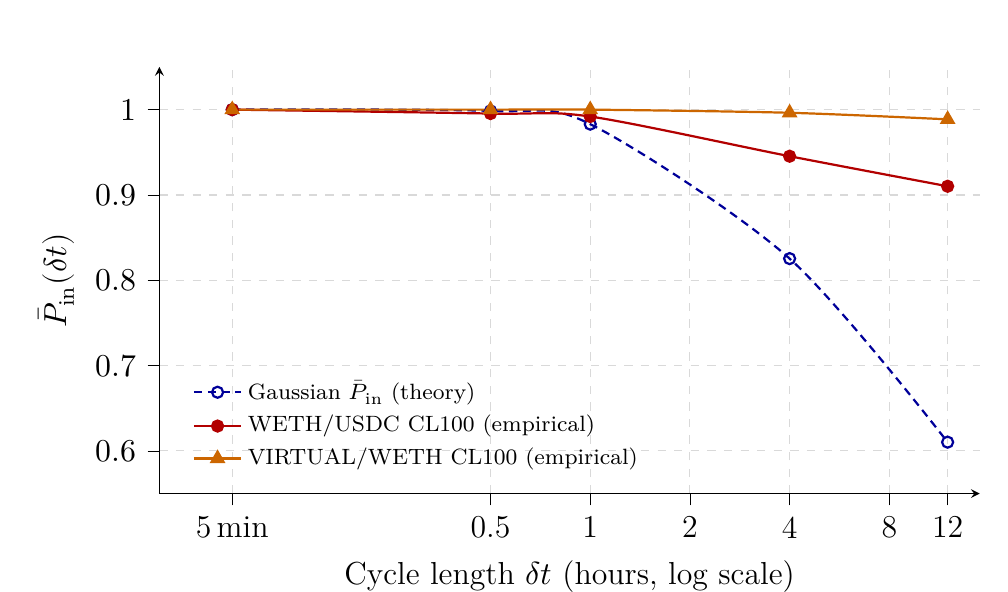
\begin{tikzpicture}
\begin{axis}[
  width=12cm, height=7cm,
  xlabel={Cycle length $\delta t$ (hours, log scale)},
  ylabel={$\bar P_{\text{in}}(\delta t)$},
  xmode=log,
  log basis x=10,
  xmin=0.05, xmax=15,
  ymin=0.55, ymax=1.05,
  xtick={0.083,0.5,1,2,4,8,12},
  xticklabels={5\,min,0.5,1,2,4,8,12},
  ytick={0.6,0.7,0.8,0.9,1.0},
  legend pos=south west,
  legend cell align=left,
  legend style={font=\footnotesize,draw=none,fill=none},
  grid=major,
  grid style={dashed,gray!30},
  axis lines=left,
  tick align=outside,
  tick style={black},
  mark options={solid},
]
\addplot[thick,blue!60!black,densely dashed,smooth,mark=o,mark size=2pt] coordinates {
  (0.083,1.0000)
  (0.5,0.9985)
  (1,0.9830)
  (4,0.8254)
  (12,0.6103)
};
\addlegendentry{Gaussian $\bar P_{\text{in}}$ (theory)}

\addplot[thick,smooth,mark=*,mark size=2pt,color=red!70!black] coordinates {
  (0.083,1.0000)
  (0.5,0.9954)
  (1,0.9919)
  (4,0.9454)
  (12,0.9102)
};
\addlegendentry{WETH/USDC CL100 (empirical)}

\addplot[thick,smooth,mark=triangle*,mark size=2.5pt,color=orange!80!black] coordinates {
  (0.083,1.0000)
  (0.5,1.0000)
  (1,1.0000)
  (4,0.9963)
  (12,0.9886)
};
\addlegendentry{VIRTUAL/WETH CL100 (empirical)}
\end{axis}
\end{tikzpicture}
\caption{Empirical vs Gaussian $\bar P_{\text{in}}$ for minimum-width positions on two Base mainnet CL100 pools. Empirical $\bar P_{\text{in}}$ exceeds the Gaussian at $\delta t > 1$\,h, leaving the parasitic ratio bound a valid upper bound under the empirical process at the relevant step in Theorem~\ref{thm:parasitic}'s derivation.}
\label{fig:pinvalidation}
\end{figure}

For the tested pools at their current volatility, the range-exit scale~(\ref{eq:exitscale}) is
\[
\delta t^* \;\approx\; \frac{(a\eta)^2}{\sigma^2} \;=\; \frac{(100 \cdot 10^{-4})^2}{(8.93 \cdot 10^{-5})^2} \;\approx\; 1.25 \times 10^4\,\text{s} \;\approx\; 3.5\,\text{h}
\]
for a minimum-width position ($a = 100$ ticks on a CL100 pool). The Gaussian in-range probability formula is therefore a reliable tool at cycle times well below this scale, which covers the original parasitic extraction attack's 2-second regime and the 10-second adversarial window discussed in~\S\ref{sec:composed}. At cycle times above $\delta t^*$, the per-position range filter of the CL gauge baseline itself already drives rewards to zero regardless of scoring function; the corrective accumulator's distinguishing contribution is in the short-cycle regime.

\subsection{Composed empirical suppression}\label{sec:composed}

Reference\cite{ryan2026c} reports parasitic extraction of $0.66\%$ of baseline under the combined minimum-width and warmup remediation against the pre-upgrade Aerodrome gauge (the unmitigated CL baseline, a CL gauge with range-aware accumulator but no width, warmup, or concentration remediations). The three corrections together therefore bound short-cycle parasitic extraction at no more than $0.66\%$ of the unmitigated CL baseline; the concentration factor provides additional width discrimination beyond the minimum-width floor, though at the measured $0.66\%$ level the marginal gain is small. Direct comparison with Aerodrome's post-upgrade step gate is deferred to \S\ref{sec:threshold}.

% ---- 6. Calibration ----
\section{Calibration from operational data}\label{sec:calibration}

Parameter values for the reference instance (Table~\ref{tab:reference}) are derived from a single-operator dataset of concentrated liquidity rebalancing on Aerodrome Base over a 38-day pre-migration window (7~March to 13~April 2026). Activity reflects a mix of autonomous policy execution by the author's CL management contracts and periodic manual position adjustments; this is not aggregate market data, and lies in the cadence tail of \cite{heimbach2022} rather than at the population median. The window ends shortly before seven pools migrated to the post-upgrade Aerodrome gauge on and after 16~April (\S\ref{sec:composed}). The dataset contains 94{,}469 rebalance events (after filtering numerical outliers from a raw 96{,}719) across 48 pools. From these, 94{,}267 consecutive-rebalance pairs lie within a 1-day inter-event cap (Tab~\ref{tab:interval}); the broader 96{,}517-pair pre-upgrade set used in Tab~\ref{tab:threshold} drops the cap to count long-tail intervals as well. Each event records the position's pre- and post-rebalance tick ranges, pre- and post-value in USD, geometric residual magnitude, and timestamp. A post-migration sub-window from those seven pools (16--21~April) provides a behavioural sanity check in~\S\ref{sec:threshold} rather than calibration data; the regime under the 10\,s gate is different.

The dataset reflects the author's tight-range rebalancing under the unconstrained pre-upgrade gauge, lying in the active-management tail of Heimbach \emph{et al.}\cite{heimbach2022} rather than at the population median. Under the proposed ramp, rational LPs lengthen cadence to raise $\bar f(\rho)$, so observed pre-constraint cadence overstates the cadence an equilibrium population would maintain. The drag values below are therefore upper bounds on drag for the active-management regime represented in the dataset; extrapolation to broader populations is not made here.

\subsection{Observed width distribution}\label{sec:calwidth}

\begin{table}[H]
\centering
\caption{Position width distribution across 94{,}469 rebalance events.}
\label{tab:width}
\begin{tabular}{@{}lr@{}}
\toprule
Quantile & Width (ticks) \\
\midrule
p25 & $67$ \\
Median & $200$ \\
p75 & $200$ \\
Mean & $176$ \\
\bottomrule
\end{tabular}
\end{table}

The median active position spans 200 ticks, with the interquartile range running from 67 to 200 ticks. The distribution shifts mid-window. Events before 8~April concentrate around a 100-tick median; from 8~April onwards positions widened for impermanent loss and fee reasons independent of gauge mechanics, lifting the median to 200 ticks. Both regimes sit in the non-capped regime of the reference concentration curve. With $w_{\text{ref}} = 1000 \times$ tickSpacing, the cap $c_{\max} = 100$ activates only at $w \leq w_{\text{ref}}/c_{\max}$, well below the observed p25 at typical active-LP tickSpacings, so the curve applies a smooth gradient across the observed distribution rather than clipping to the cap. A tighter cap, for instance $c_{\max} = 25$, activates at $w \leq w_{\text{ref}}/25 = 40 \times$ tickSpacing, which is also below the observed p25; neither choice clips the bulk of the observed distribution, and the calibration of \S\ref{sec:calinterval} is unaffected by which value is taken. Resolution of the cap choice against operator data outside this dataset's active-management tail is left to a trilogy-wide calibration audit.

\subsection{Rebalance interval distribution}\label{sec:calinterval}

\begin{table}[H]
\centering
\caption{Rebalance interval distribution across 94{,}267 consecutive-rebalance pairs (1-day cap).}
\label{tab:interval}
\begin{tabular}{@{}lrr@{}}
\toprule
Quantile & Seconds & Minutes \\
\midrule
p25 & $110$ & $1.8$ \\
Median & $368$ & $6.1$ \\
p75 & $958$ & $16.0$ \\
p95 & $4{,}682$ & $78.0$ \\
Mean & $1{,}201$ & $20.0$ \\
\bottomrule
\end{tabular}
\end{table}

The median rebalance interval is 368\,s (approximately 6 minutes), with p25 at 110\,s and p75 at 958\,s. The lower tail reflects reactive rebalancing in volatile conditions; the upper tail reflects steady-state maintenance.

This distribution informs the warmup period $W$. Under Theorem~\ref{thm:legit}, the freshness drag for a legitimate LP is $W/(2\rho)$. At the observed median $\rho_{\text{legit}} = 368$\,s with $W = 20$\,s, the equilibrium freshness $f_{\text{eq}} = 1 - W/(2\rho_{\text{legit}}) \approx 0.973$, and a 2-second parasitic cycle attains $\bar f(2) = 2/(2 \cdot 20) = 0.05$. Substituting into Cor~\ref{cor:short}, $\mathbb{E}[R^{\text{corr}}_{\text{op}}]/\mathbb{E}[R^{\text{std}}_{\text{op}}] \leq 0.051 \cdot c(w_{\min})/c_{\text{ref}} + O(N^{-1/2})$ at the 2-second cycle. The sign and magnitude of $c(w_{\min})/c_{\text{ref}}$ depend on the population's typical width and are an empirical input not measured in this paper. The corresponding legitimate-LP drag is $W/(2\rho_{\text{legit}}) = 2.7\%$. Shorter warmups ($W \approx 10$\,s) halve the drag at the median to 1.4\% with marginally weaker suppression of sub-second cycles. Longer warmups ($W \approx 60$\,s, proposed in \cite{ryan2026c}) yield 8.2\% drag at the observed median; the choice within $[10, 60]$\,s is a deployment trade-off between drag at the median and short-cycle suppression. All drag figures are upper bounds for the active-management regime, per the equilibrium-response argument at the start of~\S\ref{sec:calibration}.

\subsection{Step-gate threshold impact on observed cadence}\label{sec:threshold}

Aerodrome's post-upgrade gauge\cite{aerodrome2026} enforces a step-function freshness penalty with \texttt{minStakeTimes} = 10\,s and \texttt{penaltyRate} = 10{,}000\,bps (full forfeit below threshold). A Foundry probe against the live CL100-WETH/VVV post-upgrade gauge (\texttt{test\_Post\-Upgrade\-Step\-Function}) measures zero rewards for $\delta t < 10$\,s and full rewards at $\delta t \geq 10$\,s, with identical per-second rate post-threshold. Figure~\ref{fig:freshness-compare} compares the step against the continuous ramp $\bar f(\delta t)$ from~(\ref{eq:fbar}). The step is stricter than the ramp below 10\,s but leaves the interval $10 \leq \delta t < 2W = 40$\,s uncovered: a strategy cycling at $\delta t = 10.1$\,s receives full reward under the production gate, while the ramp applies $\bar f(10.1) \approx 0.25$ suppression in the same regime.

\begin{figure}[H]
\centering
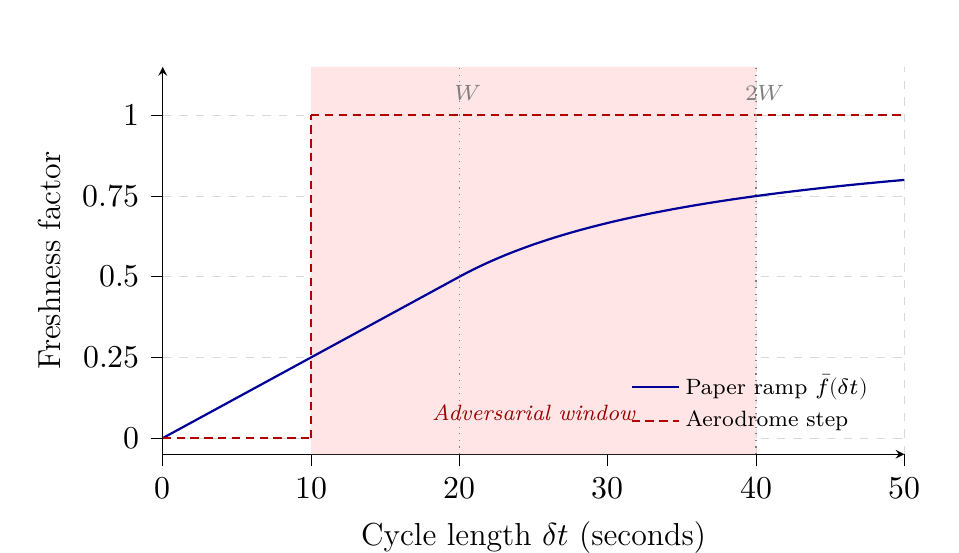
\begin{tikzpicture}
\begin{axis}[
  width=11cm, height=6.5cm,
  xlabel={Cycle length $\delta t$ (seconds)},
  ylabel={Freshness factor},
  xmin=0, xmax=50, ymin=-0.05, ymax=1.15,
  xtick={0,10,20,30,40,50},
  ytick={0,0.25,0.5,0.75,1.0},
  legend pos=south east,
  legend cell align=left,
  legend style={font=\footnotesize,draw=none,fill=none},
  grid=major,
  grid style={dashed,gray!30},
  axis lines=left,
  tick align=outside,
  tick style={black},
]
\addplot[fill=red!10,draw=none,forget plot] coordinates {(10,-0.05) (40,-0.05) (40,1.15) (10,1.15)} \closedcycle;
\node[font=\footnotesize\itshape,text=red!60!black] at (axis cs:25,0.08) {Adversarial window};

\addplot[thick,blue!60!black,domain=0:20,samples=50] {x/40};
\addplot[thick,blue!60!black,domain=20:50,samples=80,forget plot] {1 - 20/(2*x)};
\addlegendentry{Paper ramp $\bar f(\delta t)$}

\addplot[thick,red!70!black,densely dashed] coordinates {(0,0) (10,0)};
\addplot[thick,red!70!black,densely dashed,forget plot] coordinates {(10,0) (10,1)};
\addplot[thick,red!70!black,densely dashed,forget plot] coordinates {(10,1) (50,1)};
\addlegendentry{Aerodrome step}

\draw[gray,dotted] (axis cs:20,-0.05) -- (axis cs:20,1.15);
\node[font=\footnotesize,text=gray] at (axis cs:20.5,1.07) {$W$};
\draw[gray,dotted] (axis cs:40,-0.05) -- (axis cs:40,1.15);
\node[font=\footnotesize,text=gray] at (axis cs:40.5,1.07) {$2W$};
\end{axis}
\end{tikzpicture}
\caption{Continuous ramp $\bar f(\delta t)$ versus Aerodrome's post-upgrade 10\,s step gate. The shaded adversarial window is uncovered by the step but receives strict suppression under the ramp.}
\label{fig:freshness-compare}
\end{figure}

Table~\ref{tab:threshold} shows the fraction of pre-upgrade rebalance intervals below each threshold $T$ and the reward treatment each band receives under (a) the continuous freshness ramp with $W = 20$\,s and (b) the 10\,s step gate.

\begin{table}[H]
\centering
\caption{Rebalance intervals below threshold $T$ and reward treatment under each gate, over 96{,}517 pre-upgrade consecutive-rebalance pairs.}
\label{tab:threshold}
\begin{tabular}{@{}rrrll@{}}
\toprule
$T$ (s) & Count $< T$ & \% & Ramp credit & Step gate \\
\midrule
$5$   & $0$        & $0.00\%$ & --                & forfeit \\
$10$  & $3{,}825$  & $4.0\%$  & $\approx 23\%$    & forfeit \\
$15$  & $9{,}325$  & $9.7\%$  & $\approx 26\%$    & full reward \\
$20$  & $9{,}939$  & $10.3\%$ & $\approx 27\%$    & full reward \\
$30$  & $12{,}679$ & $13.1\%$ & $\approx 35\%$    & full reward \\
$60$  & $17{,}912$ & $18.6\%$ & $\approx 56\%$    & full reward \\
\bottomrule
\end{tabular}
\end{table}

4.0\% of intervals fall below the 10\,s threshold (12.7\% on WETH/USDC CL100 specifically), reflecting tight range-tracking in volatile conditions rather than gauge response since the dataset is pre-upgrade. The step forfeits these rewards in full; the ramp pays approximately 23\% at the mean sub-10\,s interval. In the $[10, 20)$\,s band (6.3\% of intervals) the step pays in full while the ramp applies graded suppression. Under the step, an LP chooses between forfeiting short-cycle rewards and throttling rebalances to at least 10\,s, the latter trading range-tracking precision for reward retention; the continuous ramp integrates the penalty over $[0, 2W]$ and imposes no such binary.

A post-migration sub-window provides a behavioural sanity check. Seven pools migrated to the post-upgrade gauge on or after 16~April (USDC/cbBTC, EURC/USDC, WETH/cbBTC, WETH/USDC at CL1; GIZA/USDC, TIBBIR/WETH, MEZO/MUSD at CL200); others stayed on the pre-upgrade gauge. Across the seven migrated pools over Apr 16--21 ($n = 666$ intervals), median cadence lengthened from 368\,s to 1{,}919\,s (approximately 32 minutes) and sub-10\,s intervals collapsed from 4.0\% to 0.2\%. Median width held at 80 ticks, consistent with the gate imposing a cadence floor rather than penalising concentration. Unmigrated pools show a separate, gate independent widening driven by a pre-existing impermanent loss adjustment and are not gate response evidence. The sample is too thin for formal calibration, but the direction matches the trade-off above.

% ---- 7. Discussion ----
\section{Discussion}\label{sec:discussion}

This section addresses what the framework does and does not cover, on three axes: operational concerns adjacent to but distinct from the scoring layer (\S\ref{sec:outofscope}); the incentive properties of the scoring function within a single pool (\S\ref{sec:incentive}); and the fit of the scoring function inside the broader ve(3,3) emission architecture (\S\ref{sec:ve33}). Limitations of the formal results and the empirical work are gathered in \S\ref{sec:limitations}; future work in \S\ref{sec:future}.

\subsection{What the framework does not address}\label{sec:outofscope}

Several adjacent concerns fall outside scope. Active management of a concentrated liquidity position is costly in time and gas, and the corrective scoring rewards the activity without supplying the keeper networks, vault abstractions, or delegation patterns that make it accessible to passive capital. Atomic rebalancing produces a geometric residual from the tick mismatch between consecutive ranges\cite{ryan2026a}; the handling of that residual is an implementation choice affecting capital efficiency but not the scoring function. Rebalances involving a token swap are exposed to MEV, and protocol-level MEV protection (private mempools, commit-reveal, post-swap slippage checks) is a distinct layer not addressed here. The emission rate, decay curve, and allocation between LPs and token holders are governance variables unrelated to the within-pool distribution this paper formalises. Cross-pool emission allocation by voter weights, bribing markets, and the broader ve(3,3) governance layer also remain unchanged here, since the present work operates strictly within a single gauge.

\subsection{Incentive compatibility}\label{sec:incentive}

The score~(\ref{eq:score}) is non-decreasing in liquidity, non-increasing in width, non-decreasing in time-since-rebalance up to the warmup-plateau transition, and zero whenever the position is out of range. At fixed population scores, an LP increases expected yield by depositing more capital, by holding a tighter range, by holding within range, and by not rebalancing more often than the ramp's full-credit threshold. These are the protocol-aligned behaviours. The alignment is direction-by-direction rather than equilibrium-optimal: intended behaviours dominate parasitic strategies within the scoring function, but the full multi-LP competitive equilibrium depends on population response and is out of scope. The accumulator's correctness inherits the gauge's existing trusted accounting of position liquidity and current tick; no additional LP-side trust assumption, allow-listing, or off-chain attestation is introduced.

\subsection{Architectural framing in ve(3,3)}\label{sec:ve33}

The scoring function applies to concentrated liquidity gauges deployed in ve(3,3) protocols. In ve(3,3)\cite{cronje2022}, emissions are a voter-directed subsidy. The inflation budget is allocated across pools by veNFT holders' votes; bribers pay voters to influence that direction; staked LPs within a pool receive emissions as payment for the liquidity voters wanted there. An unstaked LP earns swap fees directly from trades through their position, while a staked LP forfeits those fees to the pool's voters in exchange for the emission share. The separation between directed subsidy (to staked LPs) and organic revenue (to voters) is built into the design.

In V2-era pools with fungible LP tokens, every staked position provides tradeable depth proportional to its token balance; staked liquidity and tradeable liquidity coincide. The Synthetix stake-proportional accumulator therefore distributes the subsidy along the criterion voters care about, and the literal mechanic (stake yields payment) matches the functional intent (real liquidity yields payment). In concentrated liquidity deployments (Slipstream, PCS V3, and analogous CL AMMs), the equivalence breaks. A staked position can be narrow, held briefly, or out of range without providing meaningful depth. The parasitic vulnerability\cite{ryan2026c} is a composition accident of porting V2-era mechanics into a CL setting where staked liquidity and serviceable depth have diverged.

This divergence is specific to ve(3,3). Uniswap V3 fee accrual is self-pricing, since a position that captures fees has served swaps, and the rewarded and protocol-valued quantities coincide without additional mechanism. Ve(3,3) separates the two by design. Staked LPs surrender fee income to voters and receive a share of a gauge-allocated emission budget computed by an independent formula. When that formula reduces to per-$L$ accrual on active tick presence, a zero-volume position still collects its share, and the directed subsidy decouples from the outcome voters paid for. The corrective framework restores the coupling by making the within-pool formula track tradeable depth directly; voting, bribing, cross-pool allocation, and the fact of emissions accruing to staked LPs all remain unchanged.

Cronje's original design\cite{cronje2022} placed no bound on voter-directed emission fraction per pool; production CL-era deployments (notably Aerodrome's per-gauge cap with cross-gauge redistribution) constrain voter direction as a defence against the extraction surface that opens when large flows meet a nominal stake scoring formula. The corrective accumulator closes that surface at the per-LP measurement level.

Aerodrome's forthcoming Predictive Allocation\cite{aerodrome2026pa}, scheduled for July 2026 with the Aero merger, replaces discrete weekly bribe voting with continuous real-time allocation in which token operators live-allocate emissions based on forward-looking forecasts of pool fee generation and are rewarded differentially by prediction accuracy. Predictive Allocation operates on cross-pool emission direction; the present analysis operates on within-pool LP distribution. The two layers compose.

\subsection{Limitations}\label{sec:limitations}

Several caveats apply. Lemma~\ref{lem:meanfield} treats per-LP scores as independent, while real LPs' scores are correlated through the shared tick trajectory; the concentration argument holds at the same order on minute-to-hour timescales where independent deposit, withdraw, and rebalance decisions dominate, but a weak-dependence extension would be needed for correlated-LP regimes. Theorem~\ref{thm:parasitic} assumes a no-drift Gaussian log-price (Appendix~\ref{app:notation}); empirical tick processes exhibit mean reversion at long horizons, and the validation in~\S\ref{sec:empirical-pin} confirms the Gaussian formula is conservative, so the parasitic extraction bound remains valid, but exact magnitudes may be overstated above the range-exit scale~$\delta t^*$.

The calibration dataset of~\S\ref{sec:calibration} comes from the author's own positions on Aerodrome (Base) over a 38-day pre-migration window, combining autonomous policy execution by the author's CL management contracts with ad-hoc manual position adjustments; it is not aggregate market data, and the width and interval distributions therefore reflect that operator's tail of active management rather than the equilibrium population, placing the calibration squarely within the active-management regime documented by Heimbach \emph{et al.}\cite{heimbach2022}. Rational LPs facing a freshness ramp would lengthen their cadence to raise $\bar f(\rho)$, so the drag figures derived from observed pre-constraint cadence are upper bounds, with equilibrium-response analysis left to future work.

The incentive analysis of~\S\ref{sec:incentive} establishes that intended behaviours weakly increase score and yield, but does not solve the full multi-LP competitive equilibrium; whether equilibrium yields under the corrective accumulator strictly dominate the standard accumulator across all population compositions remains open. Finally, the analysis is within-pool, with cross-pool emission allocation, voting markets, and bribery mechanics\cite{lloyd2023} sitting at a separate layer and out of scope.

\subsection{Future work}\label{sec:future}

The framework admits several extensions. Concentration curves beyond the reciprocal of Table~\ref{tab:reference} (concave-then-flat, exponential-tail, or volatility-aware shapes) preserve the shape conditions on $c$ and could improve the population-typical drag bound. An equilibrium-optimal calibration of $W$ replacing the upper-bound calibration of \S\ref{sec:calinterval}, and a multi-pool extension addressing cross-gauge interactions, would round out the framework. A weak-dependence extension of Lemma~\ref{lem:meanfield} would relax the independence assumption flagged in \S\ref{sec:limitations}.

% ---- 9. Conclusion ----
\section{Conclusion}\label{sec:conclusion}

This paper specifies a within-pool scoring function for ve(3,3) concentrated liquidity gauges by attaching three multiplicative factors, a concentration weight, a freshness weight, and an in-range indicator, to each position's nominal liquidity in the Synthetix accumulator.

Three results characterise the function. Under a Brownian log-price and a steady-state mean-field legitimate population, the ratio of corrective to standard-gauge parasitic revenue is bounded above by a freshness ratio times a concentration ratio plus a mean-field error term (Theorem~\ref{thm:parasitic}); under the same hypotheses, the corresponding ratio on a legitimate LP is the analogous product up to mean-field error (Theorem~\ref{thm:legit}). Within the abstract product family over the three corrections, the full three-factor function is the only member that closes the three pathways of Definition~\ref{def:pathways} (Theorem~\ref{thm:mincomplete}); this is the only result that does not invoke the price model or population statistics. On CL gauge deployments the indicator is already supplied by the baseline accumulator, leaving the concentration and freshness factors as the novel corrections.

The empirical work is consistency evidence at three layers, not a population study. The Foundry suite reproduces the predicted score ratios, decay schedule, and zero out-of-range scores on live Aerodrome Slipstream state and on three independent CL codebases (\S\ref{sec:empirical}). Lemma~\ref{lem:pin}'s Gaussian in-range probability agrees with empirical $\bar P_{\text{in}}$ on two Aerodrome pools at short horizons and is exceeded by it at long horizons, leaving the parasitic ratio bound on the safe side of empirical departures. A single-operator dataset of 94{,}469 rebalance events fixes the warmup at $W \in [10, 30]$\,s with median legitimate-LP drag of 1.4--2.7\% in the active-management regime measured (\S\ref{sec:calibration}).

The algebraic change is local: the Synthetix accumulator's $L_i/\sum_j L_j$ becomes $S_i/\sum_j S_j$. The corrective $S_i$ is the proxy for tradeable depth proposed and characterised here; the distance between the proxy and the underlying quantity is bounded by the population statistics in Theorems~\ref{thm:parasitic}--\ref{thm:legit}. What this paper does not do: solve the multi-LP competitive equilibrium, extend Lemma~\ref{lem:meanfield} to dependent regimes, or address cross-pool emission allocation. Those are listed in \S\ref{sec:future}.

% ---- References ----
\begin{thebibliography}{9}

\bibitem{ryan2026c}
Ryan, K.R. ``Parasitic Liquidity: Emission Extraction via Non-Functional Concentrated Liquidity Positions.'' \emph{SSRN Working Paper} (2026) \url{https://doi.org/10.2139/ssrn.6510118}.

\bibitem{synthetix2019}
Synthetix. ``StakingRewards Accumulator Pattern (\texttt{rewardPerToken} / \texttt{earned}).'' Canonical instance verified on-chain as \texttt{CurveRewards} at \texttt{0xDCB6A51eA3CA5d3Fd898Fd6564757c7aAeC3ca92} (MIT, Solidity 0.5.16) (2019) \url{https://etherscan.io/address/0xDCB6A51eA3CA5d3Fd898Fd6564757c7aAeC3ca92\#code}.

\bibitem{egorov2019}
Egorov, M. ``StableSwap: Efficient Mechanism for Stablecoin Liquidity'' (2019) \url{https://berkeley-defi.github.io/assets/material/StableSwap.pdf}.

\bibitem{adams2021}
Adams, H., Zinsmeister, N., Salem, M., Keefer, R., Robinson, D. ``Uniswap v3 Core.'' \emph{Uniswap Labs Technical Whitepaper} (2021) \url{https://uniswap.org/whitepaper-v3.pdf}.

\bibitem{cronje2022}
Cronje, A. ``Solidly: Preparation for Launch.'' \emph{Medium} (2022). Original post deleted; archived 29 April 2022 at {\def\UrlBreakPenalty{100}\def\UrlBigBreakPenalty{100}\url{https://web.archive.org/web/20220429052133/https://andrecronje.medium.com/solidly-preparation-for-launch-8e653ce8a428}}.% over-column URL: breaks allowed (C26 exception).

\bibitem{ryan2026a}
Ryan, K.R. ``The Geometric Siphon: Emergent Capital Reallocation in Concentrated Liquidity Portfolios.'' \emph{SSRN Working Paper} (2026) \url{https://doi.org/10.2139/ssrn.6374838}.

\bibitem{ryan2026b}
Ryan, K.R. ``The Geometric Siphon II: Directional Properties.'' \emph{SSRN Working Paper} (2026) \url{https://doi.org/10.2139/ssrn.6481498}.

\bibitem{heimbach2022}
Heimbach, L., Schertenleib, E., Wattenhofer, R. ``Risks and Returns of Uniswap V3 Liquidity Providers.'' \emph{Proceedings of the 4th ACM Conference on Advances in Financial Technologies (AFT '22)} (2022) \url{https://doi.org/10.1145/3558535.3559772}.

\bibitem{hasbrouck2025}
Hasbrouck, J., Rivera, T.J., Saleh, F. ``An Economic Model of a Decentralized Exchange with Concentrated Liquidity.'' \emph{Management Science} (2025, forthcoming) \url{https://doi.org/10.1287/mnsc.2024.04510}.

\bibitem{cartea2024}
Cartea, \'A., Drissi, F., Monga, M. ``Decentralized Finance and Automated Market Making: Predictable Loss and Optimal Liquidity Provision.'' \emph{SIAM Journal on Financial Mathematics} (2024, forthcoming) \url{https://doi.org/10.1137/23M1602103}.

\bibitem{milionis2022b}
Milionis, J., Moallemi, C.C., Roughgarden, T., Zhang, A.L. ``Automated Market Making and Loss-Versus-Rebalancing.'' \emph{arXiv preprint} (2022) \url{https://arxiv.org/abs/2208.06046}.

\bibitem{lloyd2023}
Lloyd, T., O'Broin, D., Harrigan, M. ``Emergent Outcomes of the veToken Model.'' \emph{arXiv preprint} (2023) \url{https://arxiv.org/abs/2311.17589}.

\bibitem{xiong2023}
Xiong, X., Wang, Z., Knottenbelt, W., Huth, M. ``Demystifying Just-in-Time (JIT) Liquidity Attacks on Uniswap V3.'' \emph{IACR Cryptology ePrint Archive}, Paper 2023/973 (2023) \url{https://eprint.iacr.org/2023/973}.

\bibitem{spearbit2023}
Spearbit. ``Velodrome Finance Security Review.'' \emph{Spearbit Portfolio} (November 2023) {\def\UrlBreakPenalty{100}\def\UrlBigBreakPenalty{100}\url{https://github.com/spearbit/portfolio/raw/master/pdfs/Velodrome-Spearbit-Security-Review-Nov23.pdf}}.% over-column URL: breaks allowed (C26 exception).

\bibitem{merkl2023}
Angle Labs. ``Merkl: Concentrated Liquidity Mechanisms.'' \emph{Merkl Documentation} (2023) {\def\UrlBreakPenalty{100}\def\UrlBigBreakPenalty{100}\url{https://docs.merkl.xyz/merkl-mechanisms/campaign-types/concentrated-liquidity-mechanisms}}.% over-column URL: breaks allowed (C26 exception).

\bibitem{aerodrome2026}
Aerodrome Finance. ``Upgrades for a Supersonic Era.'' \emph{Medium} (2026) \url{https://medium.com/@aerodromefi/upgrades-for-a-supersonic-era-1861487f40c6}.

\bibitem{aerodrome2026pa}
Aerodrome Finance. ``The Economic Case for Aero.'' \emph{aero.xyz} (2026) \url{https://aero.xyz/articles/aero-economic-case/}.

\end{thebibliography}

% ---- Appendices ----
\appendix
\titleformat{\section}[block]{\Large\bfseries}{Appendix \thesection:\quad}{0pt}{}
\titlespacing*{\section}{0pt}{18pt}{8pt}

\section{Notation and setup}\label{app:notation}

{\scriptsize
\renewcommand{\arraystretch}{0.95}
\begin{longtable}{@{}cL{8.5cm}@{}}
\caption{Notation for the formal analysis.}\label{tab:notation}\\
\toprule
Symbol & Meaning \\
\midrule
\endfirsthead
\multicolumn{2}{@{}l}{\emph{Table~\ref{tab:notation} (continued)}}\\
\toprule
Symbol & Meaning \\
\midrule
\endhead
\midrule
\multicolumn{2}{r@{}}{\emph{continued on next page}}\\
\endfoot
\bottomrule
\endlastfoot
\addlinespace[3pt]
\multicolumn{2}{@{}l}{\textbf{Price process and time}} \\
\addlinespace[3pt]
$X(t)$ & log-price of the pool, $\log P(t)$ \\
$\tau(t)$ & pool tick, $X(t)/\eta$ \\
$\eta$ & tick-to-log-price scaling, $\log(1.0001)$ \\
$\sigma$ & log-price volatility per $\sqrt{\text{second}}$ \\
$\delta t$ & cycle length (parasitic cycle, or generic interval $[0, \delta t]$) \\
$\rho$ & rebalance interval of a specific (legitimate) LP \\
$\rho_{\text{legit}}$ & population-typical legitimate-LP rebalance interval \\
$\delta t^*$ & range-exit cycle length scale, $(a\eta)^2/\sigma^2$ \\
$\Delta t$ & accumulator checkpoint time-step in the standard gauge formula (\S\ref{sec:properties}) \\
\addlinespace[8pt]
\multicolumn{2}{@{}l}{\textbf{Position geometry}} \\
\addlinespace[3pt]
$w$ & position width (in ticks) \\
$w_{\min}$ & minimum permissible width \\
$w_{\text{ref}}$ & reference width in $c(w) = \min(c_{\max}, w_{\text{ref}}/w)$ \\
$a$ & half-width of a position of width $w$, $a := w/2$ \\
$L$ & nominal liquidity \\
$L_{\text{op}}$ & operator-side (parasitic) position liquidity \\
$L_{\text{legit}}$ & legitimate-LP position liquidity \\
$L_p(s)$ & total in-range pool liquidity at time $s$ (matching GS notation) \\
$\bar L_p$ & expected total in-range pool liquidity, $\mathbb{E}[L_p(s)]$ \\
\addlinespace[8pt]
\multicolumn{2}{@{}l}{\textbf{Scoring factors}} \\
\addlinespace[3pt]
$c(w)$ & concentration weight (non-increasing in $w$) \\
$c_{\max}$ & concentration cap \\
$c_{\text{ref}}$ & population-averaged concentration of in-range legitimate LPs \\
$f(x)$ & freshness weight (non-decreasing in $x$, valued in $[0,1]$) \\
$\bar f(\delta t)$ & time-averaged freshness over $[0, \delta t]$ \\
$\tilde f(\rho)$ & in-range-weighted freshness time-average over $[0, \rho]$, eq.~(\ref{eq:tildef}) \\
$f_{\text{eq}}$ & equilibrium freshness for the legitimate population, $\bar f(\rho_{\text{legit}})$ \\
$W$ & freshness warmup period \\
$f_0$ & freshness floor \\
$\Delta_{\min}$ & minimum displacement enforced for a freshness-clock reset (App.~\ref{app:auxiliary}) \\
$P_{\text{in}}(s)$ & pointwise in-range probability at time $s$ for a static parasitic position \\
$\bar P_{\text{in}}(\delta t)$ & time-averaged in-range probability over $[0, \delta t]$ (Lemma~\ref{lem:pin}) \\
$P_{\text{in,legit}}(s)$ & pointwise in-range probability at time $s$ for a legitimate LP \\
$S_i(t)$ & per-position score under the corrective function \\
$S_{\text{total}}(t)$ & total score, $\sum_j S_j(t)$ \\
$S^K$ & member of the abstract scoring family $\mathcal{F}$ for $K \subseteq \{c, f, \mathbf{1}\}$ \\
$\mathcal{F}$ & abstract product family of scoring functions \\
\addlinespace[8pt]
\multicolumn{2}{@{}l}{\textbf{Revenue and population}} \\
\addlinespace[3pt]
$\lambda$ & gauge reward rate (emissions per unit time) \\
$R^{\text{std}}_{\text{op}}, R^{\text{corr}}_{\text{op}}$ & parasitic-position revenue under the CL baseline / corrective accumulator \\
$R^{\text{std}}_{\text{legit}}, R^{\text{corr}}_{\text{legit}}$ & legitimate-LP revenue under the CL baseline / corrective accumulator \\
$R^K_{\text{op}}$ & operator-strategy revenue under scoring function $S^K \in \mathcal{F}$ \\
$N$ & number of LPs in the pool \\
\addlinespace[8pt]
\multicolumn{2}{@{}l}{\textbf{Operational terms}} \\
\addlinespace[3pt]
\emph{tradeable depth} & in-range concentrated liquidity at the active tick over the cycle, weighted by holding time (\S\ref{sec:background}) \\
\emph{legitimate LP} & a position with $w \geq w_{\min}$, $\rho \geq W$, held statically over $[0, \rho]$ (\S\ref{sec:background}) \\
$S^K$ closes $P$ & no strategy admissible under $S^K$ witnesses the existential condition defining pathway $P$ (\S\ref{sec:mincomplete}) \\
\end{longtable}
}

\subsection*{Price process}

The pool's log-price $X(t) = \log P(t)$ follows a standard Brownian motion with volatility $\sigma > 0$ per $\sqrt{\text{second}}$, starting at $X(0) = 0$. The tick $\tau(t)$ tracks $X(t)/\eta$ where $\eta := \log(1.0001)$ is the tick-to-log-price scaling. The no-drift simplification is standard\cite{milionis2022b}; conservativeness of empirical departures at longer horizons is established and validated in~\S\ref{sec:empirical-pin}.

\subsection*{Baseline revenue}

For a position $p$ over interval $[0, \delta t]$, the concentrated liquidity gauge's per-position accumulator pays
\[
R^{\text{std}}_{\text{op}}(\delta t) \;=\; \lambda L_{\text{op}} \int_0^{\delta t} \frac{\mathbf{1}[\tau(s) \in \text{range}_{\text{op}}]}{L_p(s)}\,ds,
\]
where $\lambda$ is the reward rate and $L_p(s)$ is the total in-range liquidity at time $s$. Write $R^{\text{corr}}_{\text{op}}(\delta t)$ for the corresponding revenue under the corrective scoring function~(\ref{eq:score}).

\subsection*{Position geometry}

$W$ denotes the warmup period; $w_{\min}$ the minimum permissible position width; a position of width $w \geq w_{\min}$ has half-width $a := w/2$. For a narrow-range position, nominal liquidity scales as $L \propto C/w$ at fixed capital $C$.

\subsection*{Derived quantities}

\noindent\emph{Pointwise in-range probability.} For a static position of half-width $a$ centred at $\tau(0)$,
\[
P_{\text{in}}(s) := 2\Phi(a\eta/(\sigma\sqrt{s})) - 1,
\]
giving the time-averaged $\bar P_{\text{in}}(\delta t; a, \sigma) := \frac{1}{\delta t} \int_0^{\delta t} P_{\text{in}}(s)\,ds$ of Lemma~\ref{lem:pin} on integration.

\noindent\emph{Time-averaged freshness.} $\bar f(\delta t) := \frac{1}{\delta t}\int_0^{\delta t} f(s)\,ds$. For the linear ramp $f(x) = \min(x/W, 1)$:
\begin{equation}\label{eq:fbar}
\bar f(\delta t) \;=\; \begin{cases} \delta t/(2W) & \delta t \leq W, \\ 1 - W/(2\delta t) & \delta t > W. \end{cases}
\end{equation}

\noindent\emph{In-range-weighted freshness.} For an LP with pointwise in-range probability $P_{\text{in,legit}}(s)$,
\begin{equation}\label{eq:tildef}
\tilde f(\rho) \;:=\; \frac{\int_0^\rho f(s)\,P_{\text{in,legit}}(s)\,ds}{\int_0^\rho P_{\text{in,legit}}(s)\,ds},
\end{equation}
used in Theorem~\ref{thm:legit}.

\noindent\emph{Active liquidity mean.} $\bar L_p := \mathbb{E}[L_p(s)]$ under steady-state mean-field conditions (Lemma~\ref{lem:meanfield}).

\subsection*{Population statistics}

$c_{\text{ref}}$ is the population-averaged concentration of in-range legitimate LPs (empirical quantity, distinct from the design cap $c_{\max}$). $\rho_{\text{legit}} \geq W$ is the population-typical legitimate-LP rebalance interval; $f_{\text{eq}} := \bar f(\rho_{\text{legit}})$ is the equilibrium freshness at that cadence. This identification holds under a single-cadence idealisation in which every legitimate LP rebalances at $\rho_{\text{legit}}$. Under heterogeneous cadences, $f_{\text{eq}}$ should be replaced by the steady-state expectation $\mathbb{E}_{\text{pop}}[f(s)]$ taken over the population's position-age distribution; the qualitative form of Theorems~\ref{thm:parasitic}--\ref{thm:legit} is unchanged, with $f_{\text{eq}}$ reinterpreted but no other modification required.

\section{Detailed derivations}\label{app:derivations}

\subsection*{Theorem~\ref{thm:parasitic}: parasitic extraction ratio bound}

The argument proceeds in four steps: (i) compute the CL-baseline expectation, (ii) compute the corrective expectation, (iii) bound the cross-integrand via Chebyshev, (iv) divide.

\noindent\emph{Step 1 (CL baseline).} The standard accumulator pays $R^{\text{std}}_{\text{op}}(\delta t) = \lambda L_{\text{op}} \int_0^{\delta t} \mathbf{1}[\tau(s) \in \text{range}_{\text{op}}] / L_p(s)\,ds$. Taking expectations and concentrating $L_p$ at $\bar L_p$ via Lemma~\ref{lem:meanfield},
\[
\mathbb{E}[R^{\text{std}}_{\text{op}}(\delta t)] \;=\; \frac{\lambda L_{\text{op}}}{\bar L_p} \int_0^{\delta t} P_{\text{in}}(s)\,ds + O(N^{-1/2}) \;=\; \frac{\lambda L_{\text{op}}}{\bar L_p} \cdot \delta t \cdot \bar P_{\text{in}}(\delta t; a, \sigma) + O(N^{-1/2}),
\]
with $P_{\text{in}}(s)$ as defined in Appendix~\ref{app:notation}.

\noindent\emph{Step 2 (Corrective).} Under the corrective scoring,
\[
R^{\text{corr}}_{\text{op}}(\delta t) \;=\; \lambda L_{\text{op}}\, c(w) \int_0^{\delta t} \frac{f(s)\,\mathbf{1}[\tau(s) \in \text{range}_{\text{op}}]}{S_{\text{total}}(s)}\,ds.
\]
Lemma~\ref{lem:meanfield} concentrates $\mathbb{E}[S_{\text{total}}(s)]$ at $\bar L_p \cdot c_{\text{ref}} \cdot f_{\text{eq}}$ in steady-state mean-field, so
\[
\mathbb{E}[R^{\text{corr}}_{\text{op}}(\delta t)] \;=\; \frac{\lambda L_{\text{op}}\, c(w)}{\bar L_p\, c_{\text{ref}}\, f_{\text{eq}}} \int_0^{\delta t} f(s)\,P_{\text{in}}(s)\,ds + O(N^{-1/2}).
\]

\noindent\emph{Step 3 (Bound the integrand).} The freshness $f$ is non-decreasing in $s$; the in-range probability $P_{\text{in}}$ is non-increasing. Chebyshev's sum inequality for anti-monotone functions gives
\[
\int_0^{\delta t} f(s)\,P_{\text{in}}(s)\,ds \;\leq\; \delta t \cdot \bar f(\delta t) \cdot \bar P_{\text{in}}(\delta t; a, \sigma),
\]
with $\bar f(\delta t)$ piecewise as in~(\ref{eq:fbar}) by direct integration of $\min(s/W, 1)$.

\noindent\emph{Step 4 (Ratio).} Dividing Step~2 by Step~1 cancels the shared $\delta t \cdot \bar P_{\text{in}}$ factor:
\[
\frac{\mathbb{E}[R^{\text{corr}}_{\text{op}}]}{\mathbb{E}[R^{\text{std}}_{\text{op}}]} \;\leq\; \frac{\bar f(\delta t)}{f_{\text{eq}}} \cdot \frac{c(w)}{c_{\text{ref}}} \;+\; O(N^{-1/2}).
\]
Since $c$ is non-increasing in $w$, $c(w) \leq c(w_{\min})$ for all admissible $w \geq w_{\min}$, giving~(\ref{eq:thm1}).

\subsection*{Theorem~\ref{thm:legit}: legitimate-LP yield equality}

The argument parallels Theorem~\ref{thm:parasitic}'s, with one structural difference: the bounding step is replaced by a direct identification with $\tilde f$, so the result is an equality rather than an inequality.

\noindent\emph{Step 1 (CL baseline).} Over a single rebalance interval $[0, \rho]$, the CL baseline pays
\[
R^{\text{std}}_{\text{legit}}[0, \rho] \;=\; \lambda L_{\text{legit}} \int_0^\rho \frac{\mathbf{1}[\tau(s) \in \text{range}_{\text{legit}}]}{L_p(s)}\,ds.
\]
Taking expectations and concentrating $L_p$ at $\bar L_p$ via Lemma~\ref{lem:meanfield},
\[
\mathbb{E}[R^{\text{std}}_{\text{legit}}] \;=\; \frac{\lambda L_{\text{legit}}}{\bar L_p} \int_0^\rho P_{\text{in,legit}}(s)\,ds + O(N^{-1/2}).
\]

\noindent\emph{Step 2 (Corrective).} Under the corrective scoring,
\[
R^{\text{corr}}_{\text{legit}}[0, \rho] \;=\; \lambda L_{\text{legit}}\,c(w_{\text{legit}}) \int_0^\rho \frac{f(s)\,\mathbf{1}[\tau(s) \in \text{range}_{\text{legit}}]}{S_{\text{total}}(s)}\,ds.
\]
Concentrating $\mathbb{E}[S_{\text{total}}(s)]$ at $\bar L_p\,c_{\text{ref}}\,f_{\text{eq}}$,
\[
\mathbb{E}[R^{\text{corr}}_{\text{legit}}] \;=\; \frac{\lambda L_{\text{legit}}\,c(w_{\text{legit}})}{\bar L_p\,c_{\text{ref}}\,f_{\text{eq}}} \int_0^\rho f(s)\,P_{\text{in,legit}}(s)\,ds + O(N^{-1/2}).
\]

\noindent\emph{Step 3 (Ratio).} Dividing cancels the shared $\lambda L_{\text{legit}}/\bar L_p$ prefactor and the $\int P_{\text{in,legit}}$ denominator from Step~1:
\[
\frac{\mathbb{E}[R^{\text{corr}}_{\text{legit}}]}{\mathbb{E}[R^{\text{std}}_{\text{legit}}]} \;=\; \frac{c(w_{\text{legit}})}{c_{\text{ref}}\, f_{\text{eq}}} \cdot \frac{\int_0^\rho f(s)\,P_{\text{in,legit}}(s)\,ds}{\int_0^\rho P_{\text{in,legit}}(s)\,ds} + O(N^{-1/2}).
\]
The integral ratio is $\tilde f(\rho)$ by definition~(\ref{eq:tildef}), giving~(\ref{eq:thm2}). The result is an equality (not an inequality) because $\tilde f$ is defined to absorb $f \cdot P_{\text{in,legit}}$ exactly; no Chebyshev step is invoked.

\subsection*{Corollary~\ref{cor:rangetracking}: range-tracking bounds}

\noindent\emph{Upper envelope.} The freshness $f$ is non-decreasing on $[0, \rho]$ and the in-range probability $P_{\text{in,legit}}$ is non-increasing (a freshly rebalanced position drifts out of range over time). Chebyshev's sum inequality for anti-monotone functions gives $\tilde f(\rho) \leq \bar f(\rho)$, and substituting into Theorem~\ref{thm:legit}'s equality,
\begin{equation}\label{eq:thm2upper}
\frac{\mathbb{E}[R^{\text{corr}}_{\text{legit}}]}{\mathbb{E}[R^{\text{std}}_{\text{legit}}]} \;\leq\; \frac{c(w_{\text{legit}})}{c_{\text{ref}}} \cdot \frac{\bar f(\rho)}{f_{\text{eq}}} \;+\; O(N^{-1/2}),
\end{equation}
with equality in the range-tracking limit $P_{\text{in,legit}}(s) \to 1$ uniformly on $[0, \rho]$.

\noindent\emph{$\epsilon$-tracking bracket.} If $P_{\text{in,legit}}(s) \geq 1 - \epsilon$ throughout $[0, \rho]$, then the integrand in $\tilde f$'s denominator is bracketed within $1 - \epsilon$ of $\rho$, and
\begin{equation}\label{eq:thm2lower}
(1 - \epsilon)\,\frac{c(w_{\text{legit}})}{c_{\text{ref}}} \cdot \frac{\bar f(\rho)}{f_{\text{eq}}} \;-\; O(N^{-1/2}) \;\leq\; \frac{\mathbb{E}[R^{\text{corr}}_{\text{legit}}]}{\mathbb{E}[R^{\text{std}}_{\text{legit}}]} \;\leq\; \frac{c(w_{\text{legit}})}{c_{\text{ref}}} \cdot \frac{\bar f(\rho)}{f_{\text{eq}}} \;+\; O(N^{-1/2}).
\end{equation}
The yield ratio converges to $(c(w_{\text{legit}})/c_{\text{ref}}) \cdot (\bar f(\rho)/f_{\text{eq}})$ as $\epsilon \to 0$.

\subsection*{Theorem~\ref{thm:mincomplete}: minimal completeness}

The proof has two directions, treated case-by-case in the three pathways of Definition~\ref{def:pathways}.

\noindent\emph{Forward direction ($K = \{c, f, \mathbf{1}\}$).} Each factor closes its pathway in isolation.

\noindent\emph{Forward, SC.} The ramp satisfies $f(s) \to 0$ as $s \to 0$, so the score and revenue under $S^{\{c,f,\mathbf{1}\}}$ vanish strictly faster than the $\Theta(\delta t)$ standard baseline. Hence $\liminf_{\delta t \to 0} R^{\{c,f,\mathbf{1}\}}_{\text{op}} / R^{\text{std}}_{\text{op}} = 0$.

\noindent\emph{Forward, OOR.} The indicator gives $\mathbf{1}[\tau \notin \text{range}_{\text{op}}] = 0$, so the score is identically zero on any out-of-range interval, and the expected revenue contribution from that interval is zero.

\noindent\emph{Forward, WA.} At fixed capital $C$ with $w \geq w_{\min}$, nominal liquidity scales as $L \propto C/w$ and the concentration factor is capped at $c_{\max}$, so per-unit-capital revenue is bounded above by $c_{\max} \cdot (\text{pool constant})$. Steepening $c$ within the cap cannot exceed this bound. Note this case carries the qualifier of the theorem footnote: at fixed $w_{\min}$ deployment with $c_{\max}$ retained, the bound holds independent of $c$'s presence.

\noindent\emph{Reverse direction ($K' \subsetneq \{c, f, \mathbf{1}\}$).} Removing each factor in turn produces a witness for the corresponding pathway.

\noindent\emph{Reverse, $f \notin K'$.} With $f_{K'} \equiv 1$, both $R^{K'}_{\text{op}}(\delta t)$ and $R^{\text{std}}_{\text{op}}(\delta t)$ scale as $\Theta(\delta t)$ as $\delta t \to 0$. Their ratio remains $\Theta(1)$, bounded away from zero; a narrow short-cycle strategy witnesses positive $\liminf R^{K'}_{\text{op}} / R^{\text{std}}_{\text{op}}$, reopening SC.

\noindent\emph{Reverse, $\mathbf{1} \notin K'$.} With $\mathbf{1}_{K'} \equiv 1$, a position deposited in range and left staked continues to accrue score after the tick drifts out; out-of-range intervals contribute strictly positive revenue, reopening OOR.

\noindent\emph{Reverse, $c \notin K'$.} With $c_{K'} \equiv 1$ and the cap $c_{\max}$ dropped alongside (per the theorem footnote), the concentration multiplier provides no narrow-width cap; an unbounded $c$ curve (e.g.\ uncapped reciprocal) makes per-unit-capital revenue divergent as $w \to w_{\min}$, reopening WA.

\section{Auxiliary results}\label{app:auxiliary}

\begin{proposition}[Rebalance-spam self-defeat]\label{prop:spam}
Under the linear freshness ramp $f(x) = \min(x/W, 1)$, an LP rebalancing continuously at interval $\rho < W$ attains time-averaged freshness $\bar f(\rho) = \rho/(2W)$, strictly less than the population equilibrium $f_{\text{eq}} = \bar f(\rho_{\text{legit}})$ whenever $\rho < \rho_{\text{legit}}$. Under Theorem~\ref{thm:legit}'s mean-field decomposition, the resulting yield ratio is reduced by the factor $\bar f(\rho)/f_{\text{eq}} < 1$ relative to operation at equilibrium cadence; rebalance spam therefore strictly reduces yield, independent of gas costs.
\end{proposition}

\begin{proof}
Direct integration: $\bar f(\rho) = \frac{1}{\rho}\int_0^\rho \min(s/W, 1)\,ds = \rho/(2W)$ for $\rho \leq W$. The function $\bar f$ is monotonically increasing in its argument (from~(\ref{eq:fbar})), so $\bar f(\rho) < \bar f(\rho_{\text{legit}}) = f_{\text{eq}}$ whenever $\rho < \rho_{\text{legit}}$. Substituting into Theorem~\ref{thm:legit}'s yield ratio gives a freshness factor strictly below unity.
\end{proof}

\begin{proposition}[Claim-timing orthogonality]\label{prop:claim-timing}
Under the Synthetix accumulator with continuous accrual $\dot R_i = \lambda\,S_i(t)/S_{\text{total}}(t)$, the reward claimable at any time $T$ is a deterministic function of the score history $\{S_i(s), S_{\text{total}}(s) : s \in [0, T]\}$ and is independent of when claim operations are invoked.
\end{proposition}

\begin{proof}
The per-position accumulator $A_i(t) := \int_0^t \lambda\,S_i(s)/S_{\text{total}}(s)\,ds$ depends only on the score history over $[0, t]$, so a rebalance at $t' < T$ cannot retroactively alter $A_i$ on $[0, t')$. The standard lazy-checkpoint implementation is piecewise of the same form, so the argument extends.
\end{proof}

\section{Foundry test descriptions}\label{app:forkmap}

Tests deploy against live Aerodrome Slipstream state on Base mainnet (WETH/USDC CL100 pool at \texttt{0xb2cc224c1c9feE385f8ad6a55b4d94E92359DC59}), using the production non-fungible position manager (NFPM) for minting and AERO as the emission token. Numerical values are single-run against live mainnet state and shift with pool state; qualitative claims (ordering, zero for out-of-range, score and emission ratios, decay schedule) hold deterministically.

\subsection*{Test 1: Concentration term}\label{app:test1}

\texttt{test\_TightRangeScoresHigher} verifies the concentration factor of \S\ref{sec:scoring}. A tight position at $2\times$ tickSpacing scores $9.70 \times 10^{17}$; a wide position at $20\times$ tickSpacing scores $4.94 \times 10^{16}$; the ratio is approximately 19.6.

\subsection*{Test 2: Emissions follow score}\label{app:test2}

\texttt{test\_TightRangeEarnsMoreEmissions} checks that pending rewards track the score ratio. The pending-reward ratio tight\,/\,wide is approximately 19.6, matching Test~1's score ratio to within rounding.

\subsection*{Test 3: Freshness decay}\label{app:test3}

\texttt{test\_FreshnessDecay} tracks the freshness factor over time. A fresh position scores $9.70 \times 10^{17}$; after 2\,h the score has decayed to $5.33 \times 10^{17}$ (55\%); after 5\,h to $9.71 \times 10^{16}$ (10\%, at the floor).

\subsection*{Test 4: Freshness library}\label{app:test4}

\texttt{test\_FreshnessMath\_Reference} verifies the freshness library against reference values of 10{,}000\,bps fresh, 5{,}513\,bps mid-decay, and 1{,}000\,bps stale (floor).

\subsection*{Test 5: In-range indicator}\label{app:test5}

\texttt{test\_OutOfRangeEarnsNothing} verifies the indicator factor of Theorem~\ref{thm:mincomplete}. An out-of-range position scores exactly 0 on live pool state.

\subsection*{Test 6: Multi-epoch accumulation}\label{app:test6}

\texttt{test\_GaugeEmissions\_TightVsWide} runs four 30-minute epochs on live Aerodrome CL100. The tight position earns $4.64 \times 10^{21}$ AERO wei, the wide position $2.36 \times 10^{20}$; the ratio is approximately 19.6, consistent with the single-block score ratio after freshness decay.

\subsection*{Test 7: Rebalance-spam self-defeat}\label{app:test7}

\texttt{test\_FreshnessMath\_RebalanceSpamSelfDefeat} verifies Proposition~\ref{prop:spam}. Time-averaged freshness at the midpoint of a 2\,s cycle equals 500\,bps (5\%); at the midpoint of a 10\,s cycle, 2{,}500\,bps (25\%). Both match $\rho/(2W)$ with $W = 20$\,s.

\subsection*{Test 8: Post-upgrade step-function}\label{app:test8}

\texttt{test\_PostUpgradeStepFunction} probes Aerodrome's post-upgrade CL100-WETH/VVV gauge. With $\texttt{minStakeTimes} = 10$\,s and $\texttt{penaltyRate} = 10{,}000$\,bps, the gauge gives zero reward for $\delta t < 10$\,s and full reward at $\delta t \geq 10$\,s, with identical per-second rate post-threshold.

\subsection*{Tests 9--11: Cross-chain replications}\label{app:test9}

Three independent codebases reproduce the concentration, freshness, and in-range indicator behaviour on chains without Flashblocks. \texttt{test\_BSC\_*} (three tests) runs against PancakeSwap V3 state on BSC (0.45\,s native blocks); tight-to-wide score ratio is approximately 11, mid-decay 54\%, stale 10\% of fresh, out-of-range score exactly 0. \texttt{test\_Thena\_*} (three tests) runs against Thena FUSION on BSC, a Velodrome/Solidly-family ve(3,3) DEX built on Algebra Integral; tight/wide score ratio approximately 11; same decay schedule; out-of-range zero. \texttt{test\_Ramses\_*} (three tests) runs against Ramses V2 on Arbitrum One, an independent V3-fork codebase with Ramses-specific \texttt{ramsesV2MintCallback} and 12-field mint signature including \texttt{veRamTokenId}; tight/wide score ratio approximately 15; same decay schedule; out-of-range zero.

\section{Empirical validation reproduction}\label{app:reproduction}

The empirical in-range probability validation in~\S\ref{sec:empirical-pin} was computed from live \texttt{Swap} event traces on Base mainnet. All \texttt{Swap} events from the target pool over a 24-hour window (block range $[\text{head} - 43200, \text{head}]$ on Base, with 2-second blocks) are pulled, with the tick decoded from the fifth 32-byte word of each event's data as a sign-extended \texttt{int24}. The events build a piecewise-constant tick function $\tau(b)$ keyed by block number, and realised volatility is estimated as $\sigma = \sqrt{\mathbb{E}[(\Delta X / \sqrt{\Delta t})^2]}$ with $X = \tau \cdot \log(1.0001)$. For each $(\delta t, w)$ pair, $N_s = 1500$ starting blocks are uniformly sampled from the trace, and for each sample $s$ the in-range fraction of $[s, s + \delta t / 2]$ is computed for a position of half-width $w/2$ centred at $\tau(s)$. The half-cycle horizon reflects a symmetric deposit-rebalance round trip of length $\delta t$ in which the position is anchored at its tick at the cycle midpoint, so the in-range measurement runs from the anchor time forward to the next rebalance opportunity rather than across the full round trip. The empirical estimate is compared to the theoretical $\bar P_{\text{in}}(\delta t; a, \sigma)$ from~(\ref{eq:pin}) by numerical integration with 400 midpoint-rule nodes. The computation runs in under a minute per pool on a standard workstation with a single RPC endpoint.

An equivalent reproduction without an RPC endpoint is available from the parquet archive of Pool \texttt{Swap} events used by the author's downstream tooling, which holds the top-50 Aerodrome CL pools across epochs 69--140 (December 2024 -- May 2026). Filtering the archive to the target pool and the matching block range reproduces the tick trajectory $\tau(b)$ used above; subsequent steps are unchanged. Running the protocol across non-overlapping 24-hour windows uniformly spaced through the archive's span on the two CL100 pools (24 windows on one pool, 23 on the other) strengthens the comparison from a single-window agreement to a window-averaged distribution. At the minimum-width slice ($w = 200$), empirical $\bar P_{\text{in}}$ exceeds the Gaussian baseline in 87.5\% or more of windows at every $\delta t \geq 1$\,h slice on both pools, with the median empirical-minus-Gaussian gap growing from $+0.02$ at 1\,h to $+0.16$ at 12\,h on the less volatile pool and from $+0.16$ at 1\,h to $+0.24$ at 12\,h on the more volatile pool. The empirical-below-Gaussian outliers concentrate in the highest-volatility windows, where the Brownian model under-predicts dispersion through jump-style increments rather than over-predicting through mean reversion. The cycle regime relevant to Cor.~\ref{cor:short} ($\delta t \leq W = 20$\,s) shows empirical and Gaussian agreement to better than three-decimal precision in every window.

\section{Fork test reproduction}\label{app:forktest}

The repository is at \url{https://github.com/g4nc0r/constructive-gauges}; the Zenodo DOI \url{https://doi.org/10.5281/zenodo.19690075} resolves to an immutable archival snapshot. The reference implementation realises equation~(\ref{eq:score}) with the parameter choices of Table~\ref{tab:reference} on a minimal Synthetix accumulator, and reproduces the fork-test results of Appendix~\ref{app:forkmap}. The suite runs against the Aerodrome Slipstream WETH/USDC CL100 pool on Base mainnet (\texttt{0xb2cc224c1c9feE385f8ad6a55b4d94E92359DC59}), with cross-chain replications on BSC and Arbitrum One. Reproduction from a clean checkout:

\begin{codeblock}\begin{verbatim}
cd foundry
git submodule update --init --recursive

# Unit tests (no RPC needed)
forge test --match-contract MathTest -vv

# Base: Aerodrome Slipstream
BASE_RPC_URL=<your_base_rpc> forge test \
    --match-contract FrameworkForkTest -vv

# BSC: PancakeSwap V3 + Thena FUSION
BSC_RPC_URL=<your_bsc_rpc> forge test \
    --match-contract 'FrameworkBSCForkTest|FrameworkThenaForkTest' -vv

# Arbitrum: Ramses V2
ARB_RPC_URL=<your_arb_rpc> forge test \
    --match-contract FrameworkRamsesForkTest -vv
\end{verbatim}\end{codeblock}

Any working public RPC endpoint on each chain is sufficient. Forge caches RPC responses, so repeat runs are fast.

Numerical values quoted in Appendix~\ref{app:forkmap} are single-run against live Base state and shift with pool state; qualitative claims hold deterministically.

\end{document}
